\documentclass[a4paper,11pt]{report}
\usepackage{color}
\usepackage[french]{babel}
\usepackage{graphicx}
\graphicspath{{figures/}}
\usepackage{array}
\usepackage{listings}
\usepackage{url}%références avec lien url
\usepackage{amsmath}
\usepackage{multicol}%plusieurs colones
\usepackage{fancyheadings} %%%%logo
\renewcommand{\baselinestretch}{1.5}%%%%interligne
\usepackage{fancyhdr} %%%%%%en-tête
\usepackage[utf8]{inputenc}%%%%utp-8 accents
\usepackage{multirow}
\usepackage{listings}%%pour faire des listes
\usepackage{lettrine}%%lettrine (grosse lettre d'entrée de chapitre)

%\pagestyle{fancy} %: Numérotation des pages.
\lhead{Sven Borden \& Eric Brunner}% :	On personnalisera cette en-tête. haut de page gauche
\chead{2M03} %: On personnalisera cette en-tête. haut de page centre
\rhead{\today} %: On personnalisera cette en-tête. haut de page droite
\lfoot{Travail de Maturité} %:	On personnalisera cette en-tête. pied de page gauche
\cfoot{\textbf{Page \thepage/\pageref{LastPage}}} %: On personnalisera cette en-tête. pied de page centre
\rfoot{Robotique} %: On personnalisera cette en-tête. pied de page droite
\renewcommand{\headrulewidth}{0.4pt} % Trace un trait de séparation de largeur 0,4 point. Mettre 0pt pour supprimer le trait.
\renewcommand{\footrulewidth}{0.4pt} %: Trace un trait de séparation de largeur 0,4 point. Mettre 0pt pour supprimer le trait.
%%\usepackage{lastpage} %%%% conteur de page, ( 1/3 ,2/3...)
\usepackage{ucs}%%%peut être pour la fraction continue
\setlength{\hoffset}{-18pt}         
\setlength{\oddsidemargin}{2.5cm} % Marge gauche sur pages impaires
\setlength{\evensidemargin}{2.5cm} % Marge gauche sur pages paires
\setlength{\marginparwidth}{0pt} % Largeur de note dans la marge
\setlength{\textwidth}{13.3cm} % Largeur de la zone de texte (17cm)
\setlength{\marginparsep}{7pt} % Séparation de la marge
\setlength{\topmargin}{0cm} % Pas de marge en haut
\setlength{\headheight}{14.5pt} % Haut de page
\setlength{\headsep}{10pt} % Entre le haut de page et le texte
\setlength{\footskip}{3cm} % Bas de page + séparation
%\setlength{\textheight}{708pt} % Hauteur de la zone de texte (25cm)
\renewcommand{\baselinestretch}{1.5}

\definecolor{colKeys}{rgb}{0,0,1} 
\definecolor{colIdentifier}{rgb}{0,0,0} 
\definecolor{colComments}{rgb}{0,0.5,1} 
\definecolor{colString}{rgb}{0.6,0.1,0.1} 

\lstset{%configuration de listings 
float=hbp,% 
basicstyle=\ttfamily\small, % 
identifierstyle=\color{colIdentifier}, % 
keywordstyle=\color{colKeys}, % 
stringstyle=\color{colString}, % 
commentstyle=\color{colComments}, % 
columns=flexible, % 
tabsize=2, % 
frame=trBL, % 
frameround=tttt, % 
extendedchars=true, % 
showspaces=false, % 
showstringspaces=false, % 
numbers=left, % 
numberstyle=\tiny, % 
breaklines=true, % 
breakautoindent=true, % 
captionpos=b,% 
xrightmargin=-2cm, % 
xleftmargin=-2cm 
} 

\begin{document}


{\fontfamily{pnc}\selectfont %%%% attention, ne pas oublier la dernière accolade en fin de texte!!!!
\title{UGV \\(Unmanned Ground Vehicle)}
\author{Sven Borden\\ \small Travail de maturité \and  Eric Brunner\\ \small Gymnase de Morges}
\date{\today \\ ~\\
\begin{centering}
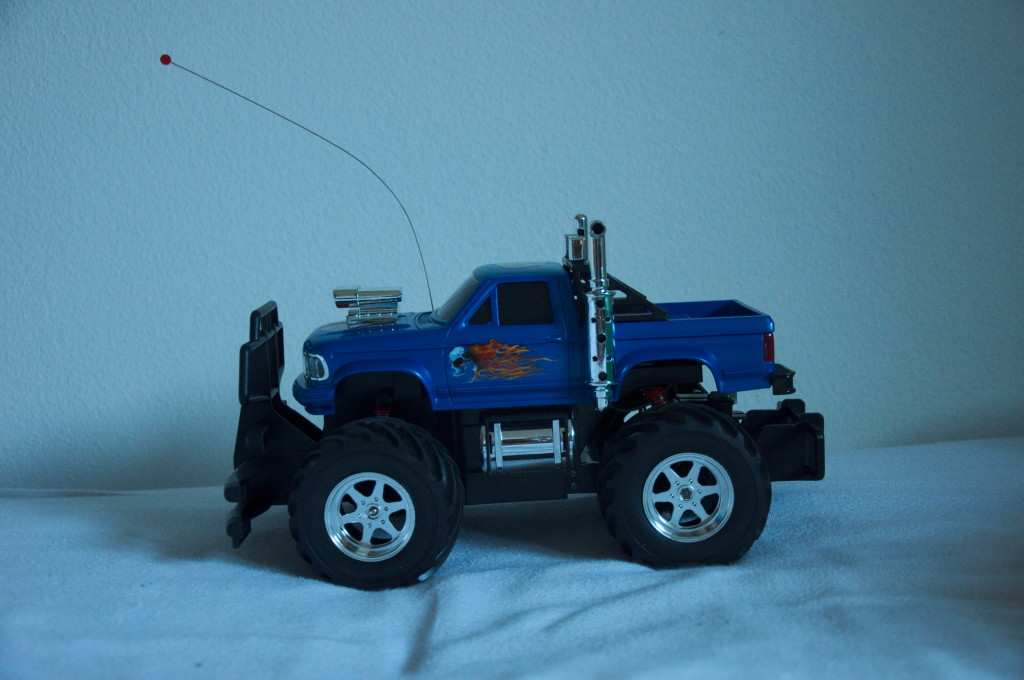
\includegraphics[width=1.0\textwidth]{DSC_8469res}
\end{centering}
\addcontentsline{lof}{figure}{\protect\numberline{}Image de courverture}
}
\maketitle



\section*{Avant-propos}
\addcontentsline{toc}{section}{\protect\numberline{}Avant-propos}

Ce dossier est le résultat de onze mois de recherches effectuées dans le cadre du travail de maturité du gymnase de Morges. Ayant déjà quelques notions en informatique, nous nous sommes dirigés  vers un domaine parallèle, la robotique. Le choix de ce sujet est dérivé des quadcopter (hélicoptères à quatres hélices). Bien que très attrayant, nous avons estimé que le travail de réalisation mécanique d'un drone volant risquait de demander trop de ressources économiques et temporelles. Nous avons préféré garder du temps pour l'aspect informatique.

%Plutot que de se lancer dans un projet dont nous savons que nous n'allons pas réussir à terminer dans les délais, nous nous sommes plutôt focalisé sur les véhicules terrestres ce qui nous a permis d'aller beaucoup plus loin que le quadcopter.

\clearpage

\section*{Remerciements}
\addcontentsline{toc}{section}{\protect\numberline{}Remerciements}
Ce projet n'aurait pu aboutir sans l'aide de nombreuses personnes. Voici l'occasion de les remercier:  Mr. Julien Dominski pour le suivi qu'il a fait pour nous ainsi que pour ses conseils en informatiques qui nous ont été grandement utiles. Mr. Denis Rochat et Mr. Phillipe Rochat pour leur disponibilité, leurs renseignements ainsi que les prêts matériels. Mr. Jean Rossier, Karl Kangur, Michaël Bolay et Mr. Marco Pagnamenta pour leurs conseils techniques, surtout à propos des plaques électroniques à imprimer. Mr. Frederic Genevey ainsi que son site edurobot.ch pour avoir promu notre projet sur son site internet. Merci à Mr. Frédéric Chaberlot pour ses prêts matériels. Mme Pauline Pidoux pour nous avoir aidé lors de la rédaction de ce travail et nous tenions aussi à remercier Stefano Varricchio pour ses informations utiles.

\clearpage

\begin{abstract}
%Parti dans l'idée de concevoir un objet déjà existant mais à moindre prix, nous avons choisi des technologies récemment sorties, ce qui fait que nous étions dans les premiers à évoluer dans ce milieu. Néanmoins, un support de développeur à toujours été là pour nous débloquer en cas de pépin. C'est entre autre grâce à eux que nous sommes parvenu a atteindre l'objectif souhaité. 

Les UGV sont des drones roulants qui sont principalement utilisés par les militaires ou la police. Ils permettent de remplir des missions qu'il serait
difficile voire impossible à faire pour l'homme ou mettant sa vie en péril. Ce type de drone existe également sur le marché des jouets, par exemple le \textit{Beewi WiFi Camera Buggy BWZ200-A1} \cite{beewi}, qui coûte septante-neuf francs.
%mais pour notre travail de maturité, son autonomie est insuffisante (une dizaine de minute tout au plus) et sa portée ne dépasse guère les 25 mètres en extérieur, ce qui rend la caméra inutile puisque le Beewi est nettement visible par le pilote. 
Notre projet ne consiste pas à fabriquer un drone ayant un fusil permettant de "dégommer" tous ce qui
bouge, mais de faire un drone de reconnaissance à moindre coûts. Les drones
existants sont soit trop cher, soit peu performants.  L'objectif de ce projet est de développer un prototype qui aurait des avantages face à un produit tel que le Beewi\cite{beewi} (une portée améliorée, une meilleure autonomie et une meilleure qualité vidéo) . En effet, si nous parvenons avoir un ensemble possédant un
véhicule tout terrain, une interface graphique claire et un guidage simple et efficace, à un prix abordable,  
nous aurions des arguments de poids face aux autres produits disponibles sur le
marché.\\
Dans la lancée de ce projet, nous nous sommes inscrit au concours
suisse de science \textit{La science appelle les jeunes}\footnote{http://fr.sjf.ch/}. Ce concours réunis presque tous les domaines, pourvu que
certains critères soient respectés. Tous les concurrents continuent un projet
qu'ils avait commencé durant leur travail de maturité/diplôme et la démarche
utilisée doit être scientifique. Ce concours pourrait, selon les résultats,
nous aider à promouvoir notre drone.  \\

%TODO
%%%%%%%%%%CONCLUSION%%%%%%%%%%%%%%%%%%%%

\end{abstract}
\addcontentsline{toc}{section}{\protect\numberline{}Résumé}
\clearpage
\tableofcontents
\clearpage
\listoffigures
%\clearpage
\listoftables 
\clearpage


\section*{Introduction}
\addcontentsline{toc}{section}{\protect\numberline{}Introduction}
Le but de ce projet est de construire un véhicule roulant que l'on peut commander à distance. Plus qu'une simple voiture télécommandée, ce drone est capable d'être contrôlé sans avoir une vue directe sur celui-ci, car il possède des capteurs tel qu'une caméra et des capteurs de distances. Ce type d'engin se nomme \textit{UGV (Unmanned Ground Vehicle)} soit "véhicule roulant sans équipage". Surtout utilisés dans l'armée, les modèles qu'on peut trouver sur le marché sont très coûteux, ils varient entre trois cents et mille trois cents francs. Notre but est donc de pouvoir construire un appareil semblable pour moins de deux cent francs. Équipé d'un répétiteur, un groupe d'UGV peut couvrir une grande surface sans mettre en danger ses pilotes puisqu'ils restent à l'écart. Il peut servir en cas de catastrophe naturelle, néanmoins, notre modèle ne peut pas rouler sur les terrains trop accidentés, mais pour corriger ce problème, il suffit tout simplement d'implémenter notre système dans un autre type de véhicule. Le développement d'une interface graphique simplifiant l'utilisation est également un but du projet. En effet, cela ne sert pas à grand chose d'avoir un drone que personne ne sait utiliser à moins de s'être entraîné durant des mois.\\
Nous avons décidé d'initier le rapport avec le chapitre concernant le hardware car il est étroitement lié à la mécanique et il permet une meilleure compréhension du reste. Ce chapitre décrit principalement l'ordinateur et le micro-contrôleur \cite{microcontroleur} embarqués sur le drone. Ensuite, le chapitre mécanique et électronique qui détaille les modifications faites à la voiture radio-commandée et les recherches faites dans ce domaine. Finalement, les deux derniers chapitres sont consacrés aux différentes versions des logiciels que nous avons créées.
\clearpage


\chapter{Hardware}


\lettrine{P}{our} réaliser ce projet, nous avons dû faire des choix au niveau du hardware.Le hardware est tout ce qui touche la partie physique du drone, néanmoins, dans ce chapitre, nous ne traiterons pas de la mécanique, ce sujet sera abordé dans le chapitre 2. Notre choix s'est porté sur deux systèmes. Le premier, l'Arduino, est un micro-contrôleur qui permet de contrôler presque ce qu'on veut grâce à un langage de programmation proche du C.\\
Le second est le Raspberry Pi, qui est un ordinateur bon marché (trente-cinq francs) qui est récemment sorti sur le marché. 


\section{Arduino}
L'Arduino \label{Arduino} \cite{Arduino} est un micro-contrôleur \textit{Open Source}, ce qui veut dire que tout le monde peut non seulement avoir accès aux plans et aux codes, mais peut aussi les modifier. Ce micro-contrôleur se programme avec un langage proche du C. 


\subsection{Choix du type d'Arduino}
Pour ce projet, nous avons choisi l'Arduino Uno, c'est l'Arduino de base.  Nous avons hésité à prendre l'Arduino Mega, mais les avantages qu'il offre ne sont pas très utiles pour notre projet. Bien qu'il ait une puissance de calcul supérieure à celle de l'Arduino Uno, il est plus coûteux et prend plus de place pour des avantages dont nous n'avons pas besoin. Dans le cadre de ce projet le coût et la place sont des facteurs déterminants.  Puisque nous n'avons pas besoin d'une grande puissance de calcul, nous avons choisi l'Arduino Uno (fig: \ref{fig:ArduinoUnoR3}). L'Arduino Uno est un micro-contrôleur.\\

\begin{figure}[h]
\begin{center}
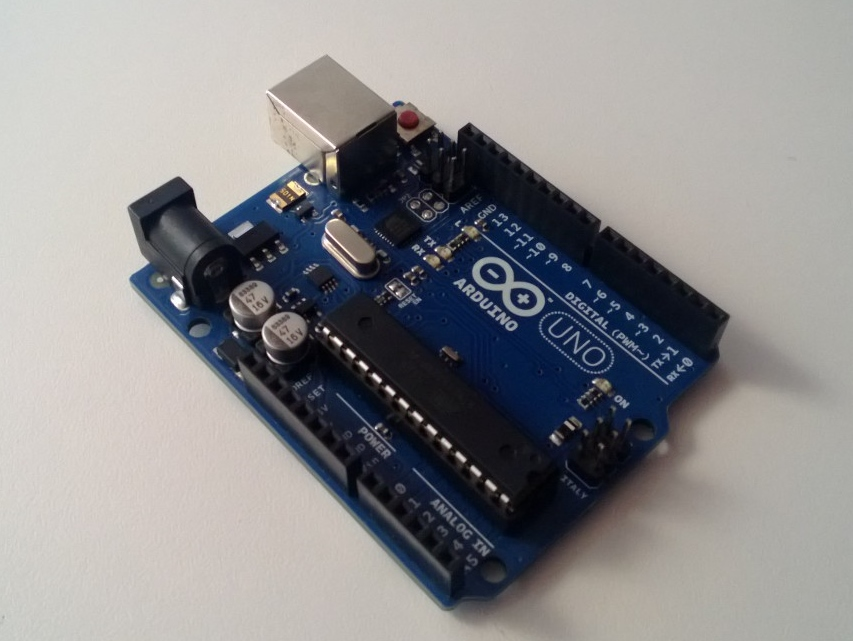
\includegraphics[scale=0.38]{arduino_uno.jpg}
\caption[Arduino Uno R3]{Arduino Uno R3\label{fig:ArduinoUnoR3}, On peut remarquer les pin  \label{pin} qui se trouvent de part et d'autre de l'Arduino. On peut remarquer au centre le micro-contrôleur ATmega328 ainsi que le port USB tout en haut de l'image}
\end{center}
\end{figure}\footnote{Les pin sont des trous où on peut y glisser des fils métalliques. Ce sont les liaisons entre le contrôleur et les senseurs}


\subsection{Détails techniques de l'Arduino}

Voici une liste des caractéristiques techniques de l'Arduino Uno R3 \cite{Arduino}:
\begin{enumerate}
\item 14 pin digitaux (signal haut ou bas) qu'on peut définit en INPUT ou en OUPUT dont 6 d'entres eux peuvent moduler le signal lorsqu'ils sont utilisé en OUTPUT
\item  6 pin analogiques  en INPUT
\item connexion USB
\item Oscillateur à quartz cadencé à 16MHz
\item Courant continu sur les pin digitaux (40mA)
\item Une sortie 3.3V et une sortie 5V en courant continu
\item 32KB de mémoire flash
\item 2KB de RAM
\item Micro-contrôleur ATmega328
\end{enumerate}
\subsection{Avantages et alternatives}
Nous n'allons pas faire une analyse approfondie des micro-contrôleurs mais il faut se rappeler qu'ils ne doivent pas faire fonctionner un système d'exploitation, mais qu'ils doivent simplement traiter des mesures et envoyer des signaux digitaux ou analogiques. Sa programmation en pseudo C le rend rapide. L'avantage de l'Arduino Uno est qu'il n'y a pas besoin de faire de soudure, les pin sont directement accessibles et on peut y glisser un fil métallique. Dans le cas où nous souhaiterions commercialiser notre produit, nous choisirons probablement l'Arduino mini car il est encore plus petit et nous pouvons directement souder les fils sur le micro-contrôleur.

\section{Raspberry Pi}
Le Raspberry Pi \cite{RaspberryPiCaracteristiques}, ou la Framboise pour les francophones, est un ordinateur de la taille d'une carte de crédit sur lequel on peut installer différents systèmes d'exploitations dérivés de UNIX/Linux. Le Raspberry Pi est acheté nu, c'est-à-dire que cet ordinateur ne possède pas d'écran, ni de clavier ou de souris, néanmoins le Raspberry Pi possède plusieurs ports où on peut brancher écran (via l'interface HDMI ou Composite), un câble Ethernet et presque ce qu'on veut grâce aux deux ports USB. Le Raspberry Pi est très intéressant non pas du point de vue de sa puissance calculatoire, mais du point de vue rapport qualité-prix (35.- CHF).

\subsection{Détails techniques du Raspberry Pi}
Voici une liste des caractéristiques techniques du Raspberry Pi modèle B \cite{RaspberryPiCaracteristiques}:
\begin{enumerate}
\item 45g environ
\item Processeur ARM1176JZF-S (ARMv6) 700MHz Broadcom 2835
\item 512Mo de RAM (sur la version B, soit celle que nous avons choisie)
\item 2 sorties vidéo (HDMI et Composite) 
\item Sortie audio stéréo Jack (3.5mm) (le son passe aussi par le HDMI en sortie 5.1)
\item Écriture et lecture possible sur une carte mémoire sous forme de carte SD (supporte les formats: SDHC, MMC et SDIO)
\item 2 ports USB 2.0 et 1 port Ethernet
\item Alimentation par câble micro USB
\item Faible consommation (5W, 5V, 1A)
\item Communication possible via les Pin GPIO
\item Décodeur permettant de lire le FullHD  1080p
\item API logiciel vidéo (OpenGL)
\end{enumerate}

\subsection{Avantages et utilisations}
Bien qu'à première vue la Framboise ne semble pas très performante, il faut prendre en compte son prix qui est bas, sa taille ainsi que les possibilités qui sont presque infinies. Les projets qu'on peut mener grâce au Raspberry Pi sont des plus varié. En effet, il peut être utilisé pour la photographie, comme base centrale d'un système de surveillance. 

\subsection{Choix de l'OS}
Une quinzaine de systèmes d'exploitations fonctionnant sur le Raspberry Pi existent. Parmi les plus connus, il y a Androïd, Arch Linux ARM et Debian/Raspbian. 
Notre choix à été porté sur Raspbian, qui est un dérivé de Debian, pour plusieurs raisons. Tout d'abord, cet OS a été développé spécialement pour le Raspberry Pi, c'est donc un OS actif et vivant continuellement développé par la communauté Raspberry. Cet OS est basé sur un environnement Linux, ce qui offre un grand nombre de libertés afin de travailler dessus. Egalement, Raspbian est gratuit, ce qui est à prendre en compte puisque nous essayons de réduire les coûts.  


\chapter{La mécanique et l'électronique}

\section{Caractéristiques du véhicule \label{TableDesc}}
\lettrine{N}{ous} nous basons sur un modèle réduit
télécommandé de type 4x4. Le tableau suivant est un inventaire de 
ses caractéristiques dans son état actuel:
\begin{table}[h!]
\begin{center}
  \begin{tabular}{|p{4cm}|p{4cm}|c|}
    \hline
    \multirow{5}{*}{Grandeurs}
    &Longueur & 35 cm \\ \cline{2-3}
    &Longueur (centre de roue \`a centre de roue)& 17 cm \\ \cline{2-3}
    &Largeur & 22 cm \\ \cline{2-3}
    &Largeur (centre de roue \`a centre de roue) & 17 cm \\ \cline{2-3}
    & Hauteur au sol & 4 cm\\ \hline
    \multirow{3}{*}{Moteur de propulsion}
    & Voltage de marche & \~{}5V - \~{}10V  \\ \cline{2-3}
    & Courant min (roue libre) & \~{}2A \\ \cline{2-3}
    & Courant max (roue bloqu\'ee) & \~{}3A \\ \hline
    \multirow{5}{*}{Servo-moteur de guidage}
    & Fabriquant & Corona \\ \cline{2 - 3}
    & Modèle & Metal gear DS558HV\\ \cline{2-3}
    & Voltage de marche & \~{}6V - \~{}7.4V  \\ \cline{2-3}
    & Courant & 300mA - 400mA \\ \cline{2-3}
    & Charge maximale & 12kg - 14kg \\  
 \hline
	\end{tabular}
\end{center}
\label{caracteristiquesDuVehicule}\caption{Caractéristiques du véhicule}
\end{table}

\section{PCB}

\begin{figure}[h!]
\centering
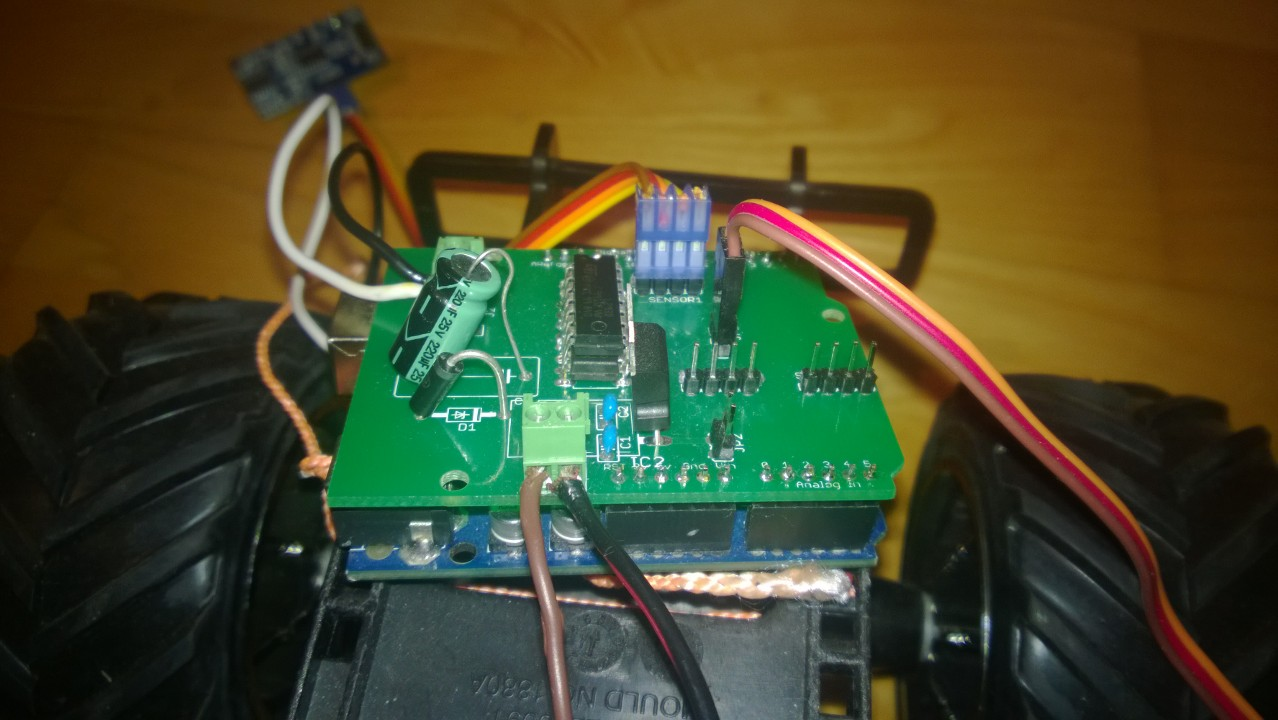
\includegraphics[width=1.0\textwidth]{figures/PCB.jpg}
    \caption{\label{PCB} Le PCB.
    }
\end{figure}

La décision de retirer l'électronique de base du véhicule télécommandé
provient d'une curiosité de comprendre comment elle est faite et surtout, du
besoin d'avoir un degré supérieur de contrôle sur la voiture. A la base, le
cerveau de la voiture se trouvait dans un petit chip. Très courant dans les
jouets radio-commandés bas de gamme, le RX2 ou similaire (fig. \ref{rx2.2}), permet d'interpréter
un signal radio et émettre des signaux pour actionner des moteurs, par
exemple. Ce micro-chip va de paire avec le TX2, qui se trouverait dans la
télécommande (TX pour "Transmit" et RX pour "Receive").


\begin{figure}[h]
\centering
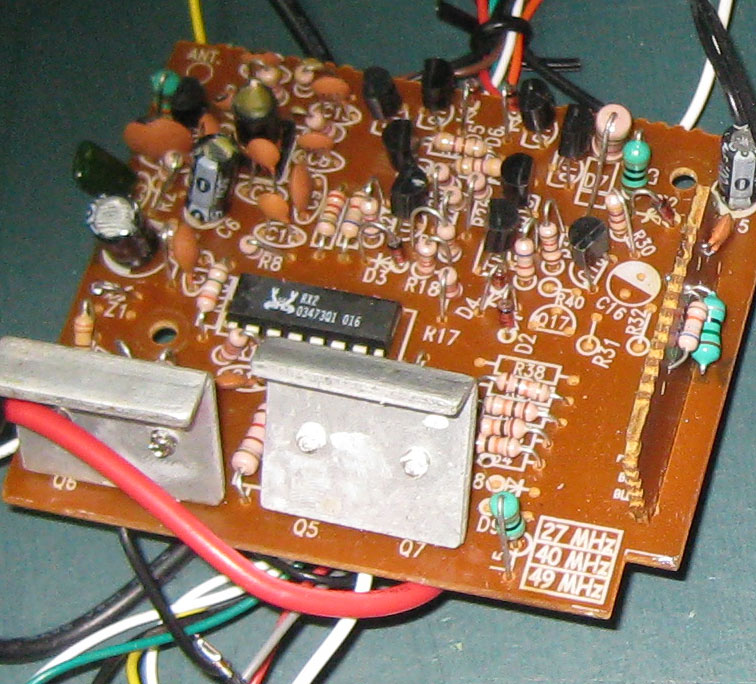
\includegraphics[width=0.6\textwidth]{figures/rx2_ex2.jpg}
    \caption[Exemple de plaque RX2]{\label{rx2.2}Exemple de plaque similaire à ce qu'on a pu trouver
      dans le véhicule.}
\end{figure}

La nature simple du chip RX2 ne lui permet que d'émettre un signal bas ou haut
(0 ou 5V), à la différence de l'Arduino qui a la possibilité de moduler le
signal (voir: \ref{servosection}). Cette caractéristique spécifique nous permet
d'avoir un large éventail de vitesses du moteur et d'angles de braquage
différents. 



\subsection{Plaque personnelle}
En attendant de recevoir la plaque sortie d'usine et pour tester une partie
design, nous avons conçu un prototype du résultat final
(fig.\ref{PPFigure}). Cette version préliminaire nous a permis de faire les
premiers
pas avec le véhicule. Elle permet de contrôler le moteur de propulsion ainsi
que le servo-moteur directionnel.
Pour une vue plus claire du prototype et une description des composants
principaux, voir la figure \ref{SchemaPlaqueMaison}. 

\begin{figure}[h]
\centering
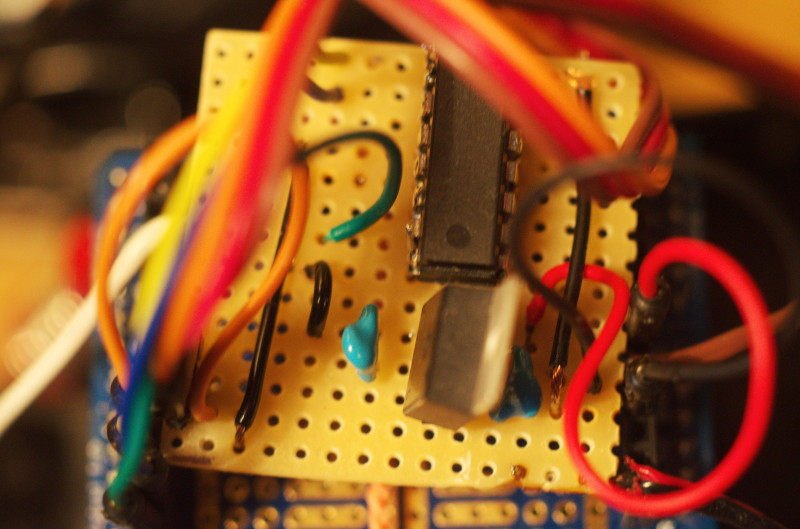
\includegraphics[width=1.0\textwidth]{figures/DSC_1116res}
    \caption[Prototype du PCB]{\label{PPFigure}Première plaque rassemblant différents composants électriques. 
    }
\end{figure}
 
\begin{figure}[h]
\centering
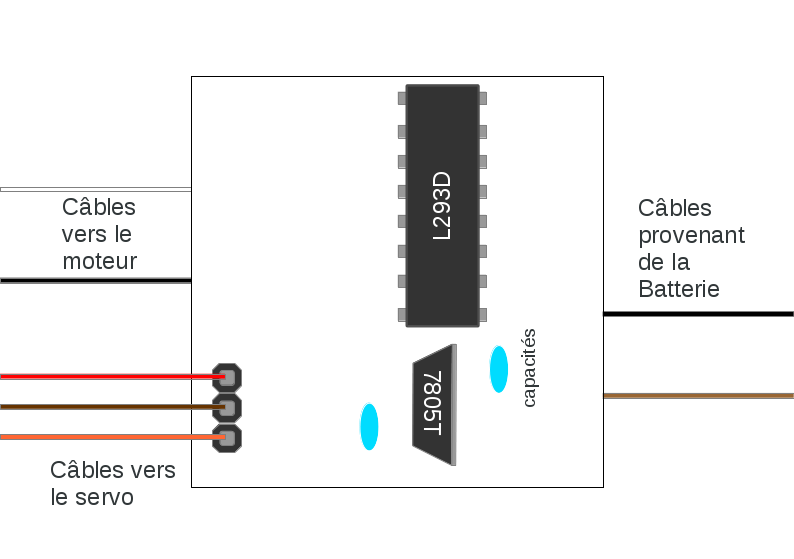
\includegraphics[width=1.0\textwidth]{figures/SchemaPlaqueMaison}
    \caption{\label{SchemaPlaqueMaison}Schéma sommaire du prototype.
    }
\end{figure}

Quelques explications sur le contenu et la conception de la plaque prototype:

\begin{enumerate}
	\item Un régulateur de voltage 5V (7805T) transforme le courant 9V de
          la batterie en 5V. 

	\item Le régulateur est entouré de capacités pour lisser d'éventuels
          sauts de tension,mais remarquez que ils seraient probablement
          inutiles lors de hauts sauts de voltage. 

	\item Un chip L293D (H-bridge (sec: \ref{h-bridge})) contrôle le
          moteur de propulsion. Ici, deux chips sont empilés, donc en
          parallèle, pour pouvoir supporter la charge importante du moteur. 
\end{enumerate}

Tous ces composants, en plus des câbles et des connecteurs vers les actuateurs
et batterie, sont soudés sur une \textit{strip-board} semblable à celle dans
la photo \ref{StripBoard}.C'est essentiellement des bandes conductrices avec des trous pour placer les
composants. les trous ont une distance standard de 0.5 pouces. Le détail des
connexions ne sera pas précisé ici, mais il ressemble évidemment 
au design de la plaque qui est illustré plus tard.   

\begin{figure}[h]
\centering
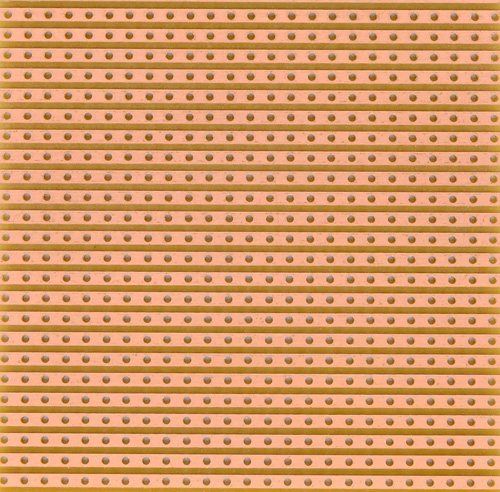
\includegraphics[width=0.3\textwidth]{figures/StripBoard}
    \caption[Strip-	board]{\label{StripBoard}Exemple de dessous de plaque de prototypage
      similaire à la notre. http://www.verotl.com/images/images/veroboards/l-01-0033.jpg
    }
\end{figure}

\subsection{Schema électronique}
Le schéma a été dessiné à l'aide d'un programme dédié gratuit (version light),
Eagle. Les symbols utilisés sont donc standardisés.
(voir fig: \ref{schemaChineComplet})

\begin{figure}[h!]
\centering
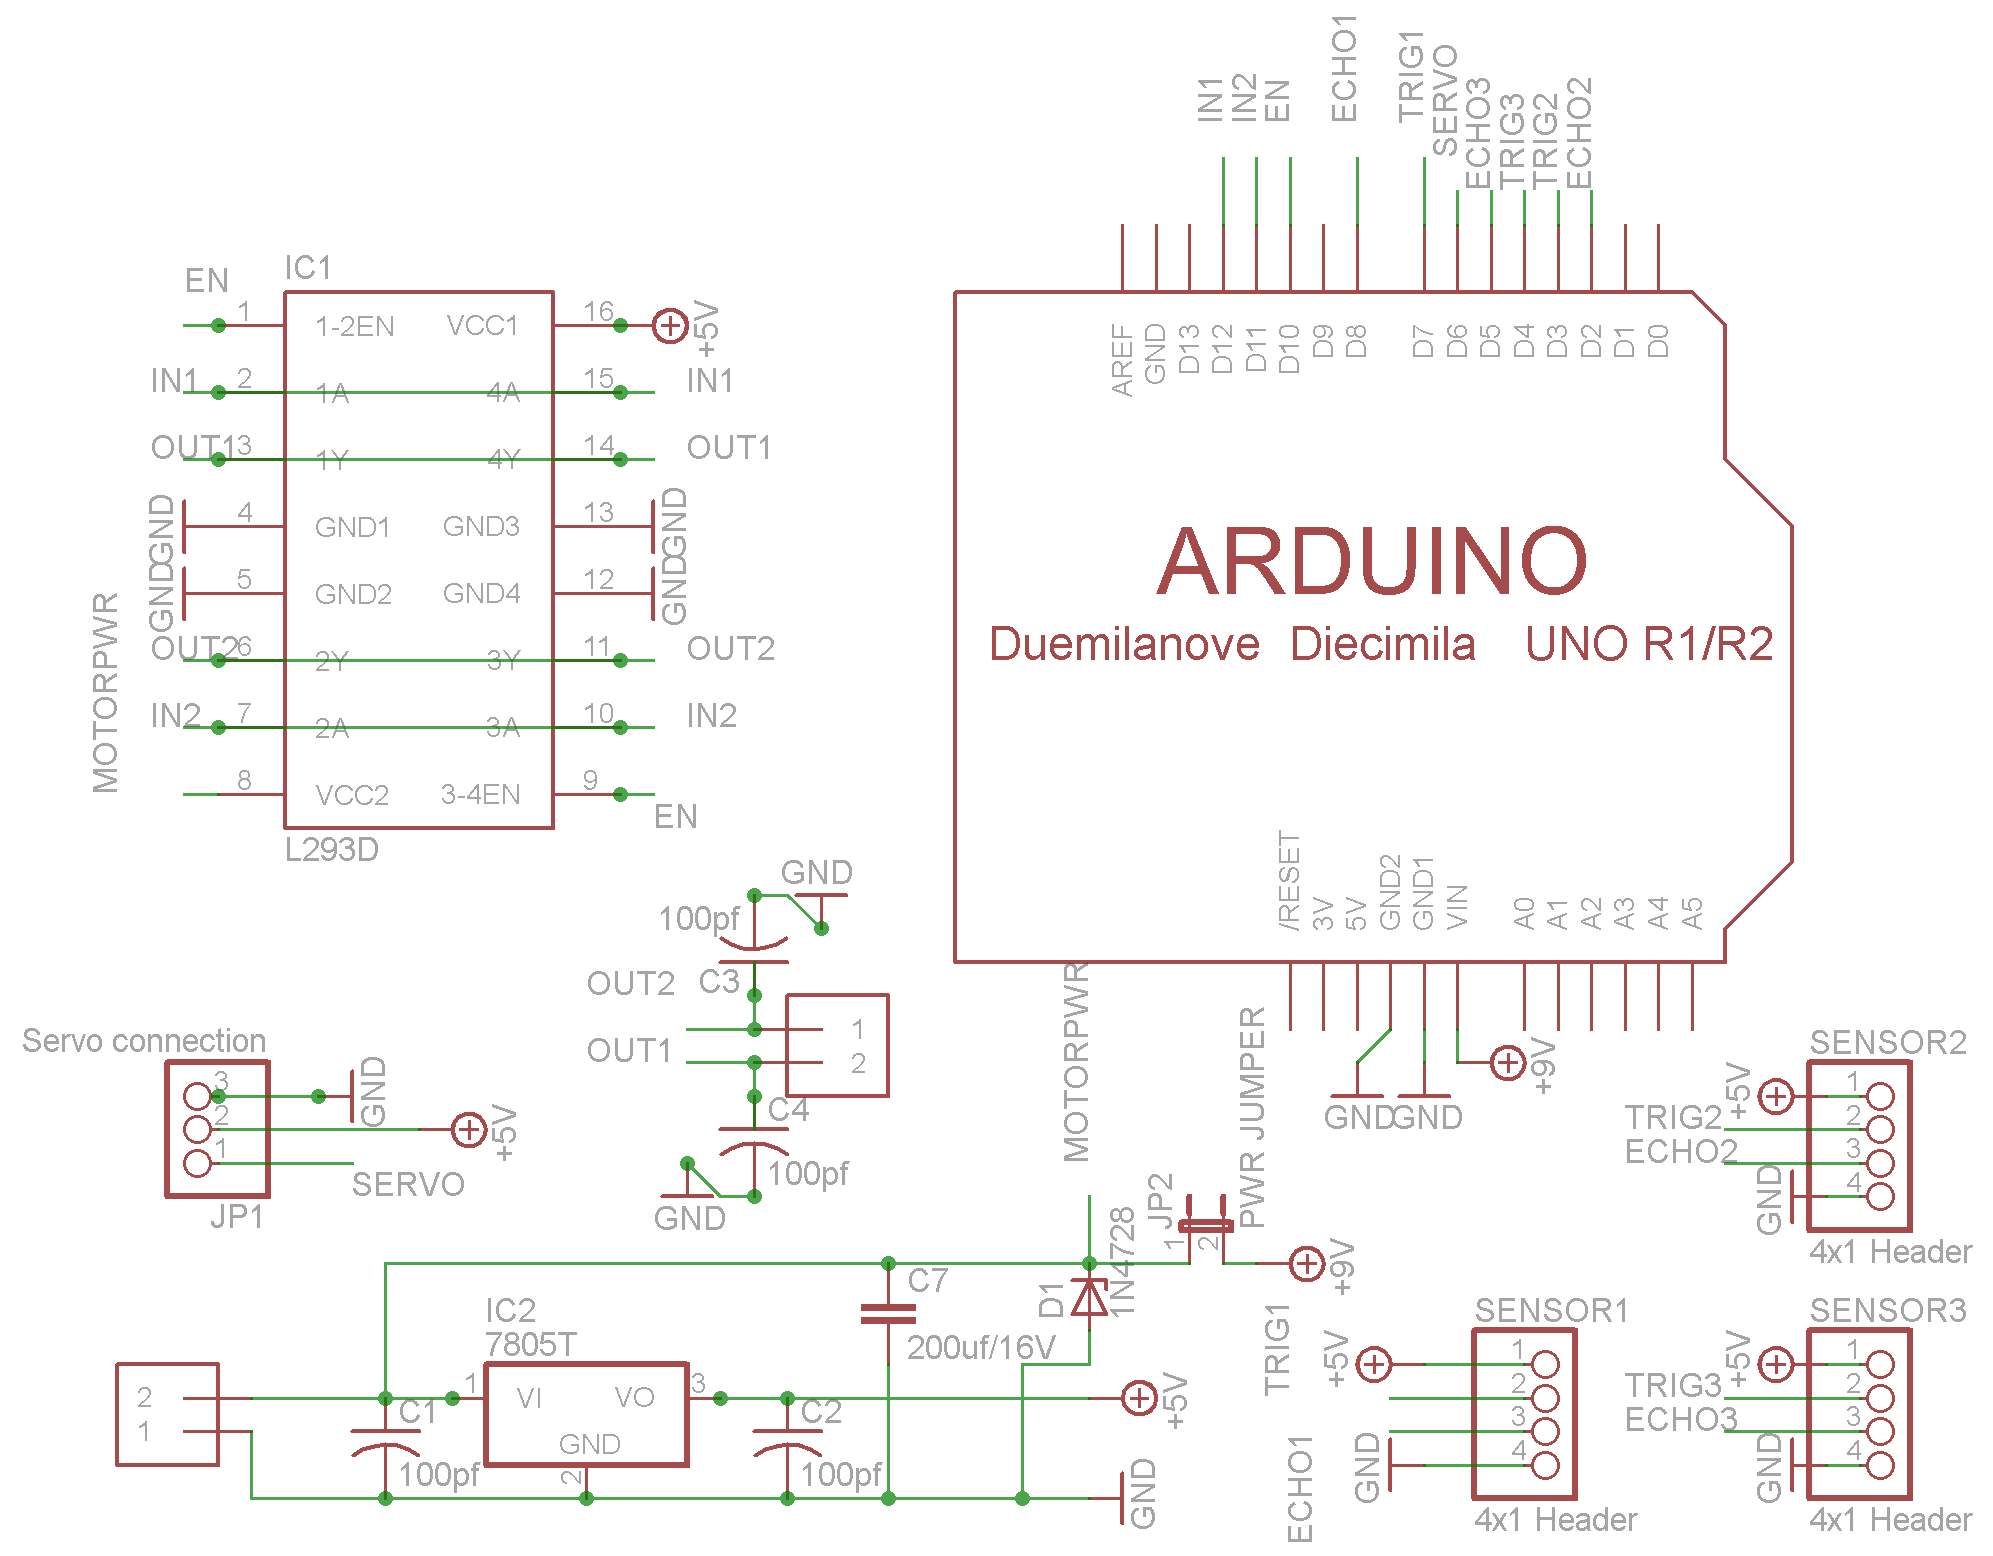
\includegraphics[angle=90, width=1.1\textwidth]{figures/schema_CHI.png}
\caption{\label{schemaChineComplet}Schéma complet du PCB
}
\end{figure}

Quelques indications pour lire le schéma:

\begin{itemize}
\item les fils portant le même nom sont connectés
\item toutes les terres sont connectées ensemble
\item Il y a un circuit 9V et un circuit 5V
\end{itemize}

\subsection{Design}
\begin{figure}[h]
\centering
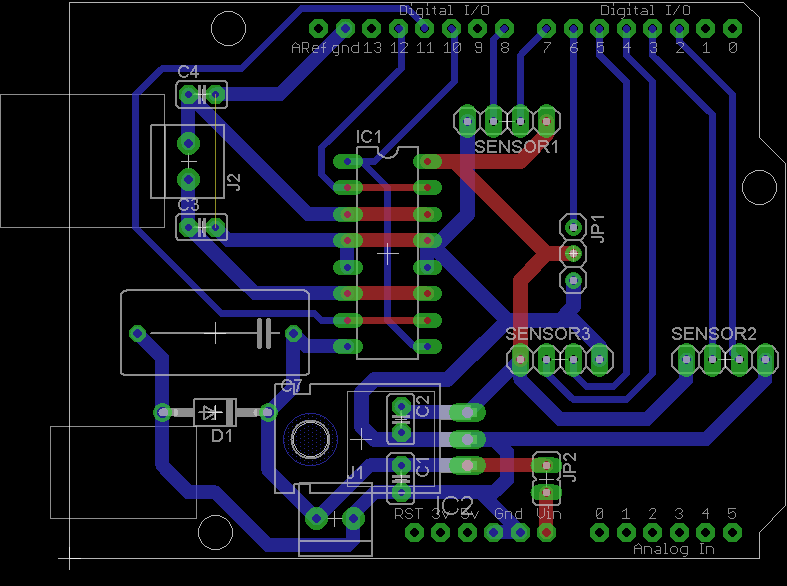
\includegraphics[width=1\textwidth]{figures/board_CHI.png}
\caption[Design final du PCB]{\label{BoardChine}Image du design final à l'ordinateur.
}
\end{figure}

Une fois le schéma dessiné, Eagle crée une plaque sur laquelle il faut disposer chaque composant. Le programme se charge de contrôler que tout est relié comme dans le schéma. Il pourrait même faire le "routing" lui-même, mais le résultat est très décevant. Des étudiants de l'EPFL nous ont conseillé de faire ça nous-mêmes. Ceci demande de la patience et de la réflexion, comme un puzzle. Nous voulions essayer d'imprimer une version à l'EPFL, il fallait donc faire un design dont les routes se trouvaient uniquement sur le derrière de la plaque (routes bleues)... Le jeu ce complique! en effet, la meilleure solution que nous avons trouvée nous laisse avec une connexion à faire à la main et un connecteur pour senseur en moins.

D'ailleurs, il faut remarquer que la plaque maison ne permet pas au robot d'interagir avec son environnement. En effet, elle peut juste contrôler des moteurs. La plaque usinée prévoit trois connecteurs pour des senseurs de distance.


\subsection{Composants}

Plus que de comprendre comment les composants sont connectés ensemble il est important de bien discerner à quoi sert chacun d'entre eux. Ici, nous détaillerons, un à un,chaque composant, ses propriétés et sa fonction.

(SCHÉMA/PHOTO qui montre où chaque composant est placé)

\begin{enumerate}
\item L293D

Le L293D est à un chip à seize pattes qui encapsule effectivement deux H-bridge comme illustré dans la section \ref{h-bridge}. Chaque moitié du pont peut fournir 0.6A de courant continu et 1.2A en pic	 \cite{l293dDataSheet}. Sachant que le moteur peut tirer jusqu'à 3A lorsque la roue est bloquée, il est clair qu'un seul de ces demi-chip est loin d'être à la hauteur. Les avis sont partagés si il est possible de mettre ces chips en parallèle (certains transistors et autres composants ne se partagent pas la charge comme prévu lorsqu'ils sont mis en parallèle), mais, basé sur les indications d'un grand producteur d'électronique pour amateurs \cite{adafruitMotorShield}, nous avons décidé d'empiler deux L293D et de mettre leurs moitiés en parallèle, ce qui s'additionne à 2.4A de courant continu et 4.8A en pic. Nous avons pu tester et valider cette configuration avec la plaque prototype. 

\item 7805T

Le 7805T est un régulateur 5V. Il approvisionne les composants fonctionnant à 5V en courant. Il peut prendre jusqu'à 35V de tension en entrée \cite{7805T}. Il faut savoir que c'est un appareil très peu efficace car la tension non utilisée est dissipée en chaleur. Il est donc nécessaire de s'assurer que le composant arrive à dissiper suffisamment de courant. Selon les graphes il a une dissipation d'environ 2.5W. Si on somme les courants des différents composants fonctionnant à 5V on trouve qu'ils requièrent environ 1A au maximum. La plus grande partie de la consommation vient du servo-moteur qui ne demande pas un approvisionnent continu. On calcule donc une dissipation de 5W (5V*1A) ce qui excède largement les spécification du composant \cite{7805T}. Mais, les tests jusqu'à ce jour montrent que il n'y a pas de problème vu que le servo-moteur n'a pas besoin d'un approvisionnement régulier. Pour être sûr on pourrait fixer un \textit{heatsink}\footnote{un \textit{heatsink} est une pièce métallique qui permet de dissiper plus rapidement la chaleur d'un composant.} sur le composant.

\item Condensateur $200\mu f$ ou $500\mu f$

Cette capacité travaille en parallèle avec la diode Zener pour lisser le signal vers le  moteur et absorber de forts sauts de tension à la suite, par
exemple, d'un blocage soudain des roues.

\item Condensateur $100pf$

Ces petites capacités servent surtout à lisser les petites variations dans le signal, connues par exemple en sortie du régulateur de voltage.

\item Diode Zener

La diode Zener a la particularité, en plus d'être une diode, d'avoir une tension seuil au-delà de laquelle elle ne remplit plus sa fonction de diode et laisse librement passer le courant. Ceci est très pratique en cas de forts sauts de tension (fig: \ref{zener}). 
\begin{figure}[h]
\centering
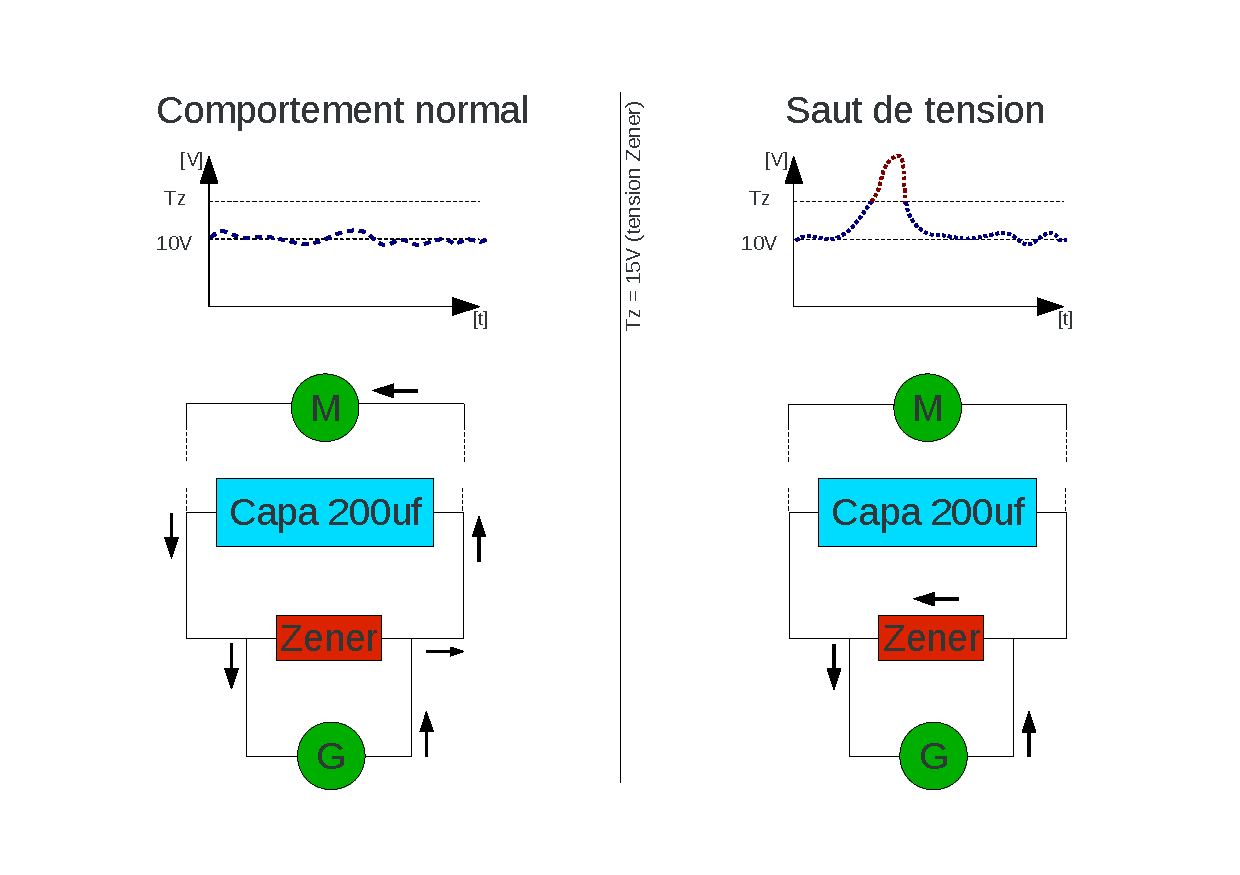
\includegraphics[width=1.0\textwidth]{CircuitZener.pdf} 
    \caption[Utilisation de la diode Zener]{\label{zener} Schéma d'un circuit ayant une diode Zener, expliquant comment cette diode permet d'éviter de griller des composants en cas de sauts de tensions. 
    }
\end{figure}


\item connecteurs senseurs

Ces connecteurs facilitent simplement la connectique et le remplacement d'un senseur au cas où il était cassé. Il y a quatre pins: deux pour l'alimentation (5v, ~15mA, pour un senseur ultrasonic HC-SR04) \cite{HC-SR04}, un pour envoyer le signal et le dernier pour recevoir l'écho.

\item connecteur servo-moteur

Tout comme les connecteurs pour senseurs à la différence qu'il n'y a que trois pins: deux pour l'alimentation (5V, ~600mA) (tab: \ref{caracteristiquesDuVehicule}

\item prises block

Ces connecteurs peuvent connecter de façon provisoire des plus gros câbles (moteur, batterie). Les câbles sont immobilisés au moyen de vis.

\end{enumerate}
\subsection{Commande et conception}
Une fois le design terminé et les composants choisis, nous pouvons envoyer
notre projet à une fabrique spécialisée. Des étudiants de l'EPFL, du club
RoboPoly, nous ont conseillé une compagnie basée en chine, SeeStudio, qui imprime des
plaques à bon prix. La procédure de perçage et d'impression est évidemment
standardisée. Le fabriquant requiert donc des fichiers bien précis à donner à
ses machines, dénommés fichiers Gerber. Ces fichiers contiennent de
l'information en coordonnées x,y et en commandes que la machine interprète. Il
serait évidemment très complexe d'écrire un tel fichier à la
main. Heureusement, le CAD que nous utilisons prévoit des scripts capable de
transformer notre design en de tels fichiers. Le fabriquant requiert
exactement huit fichiers différents, stockés dans un zip et envoyés avec la commande.  


\section{Système de guidage}


\subsection{Système directionel initial}
Dans son état initial, le système de guidage pouvait se comparer à un
servo-moteur très rudimentaire. Il en comptait toutes les caractéristiques, mais en
un état simplifié, en particulier le système de positionnement. Dans un servo-moteur
classique, il s'agit d'un potentiomètre (résistance variable) qui permet
de savoir en tout moment la position de la corne \footnote{La corne est le bras qui sort du servo-moteur et qui permet de déplacer des masses}. Par contre, dans le cas de
la voiture, un système de balais (voir image) assure cette tâche. Il en
résulte une identification de position très basique: gauche,devant ou
droite.\\
(ins\'erer images)\\
Sachant que nous avons retiré l'électronique de la voiture, il nous restait
deux possibilités: utiliser le système de guidage rudimentaire, mais
déjà en place ou tout remplacer avec un servo-moteur plus conventionnel.\\
Apr\`es beaucoup de temps perdu à tenter de contrôler le guidage de base
avec notre électronique importée, nous avons décidé de passer à un servo-moteur. Nous avons
acheté un puissant servo-moteur de haute qualité chez une connaissance qui en
avait commandé un gros lot pour la modique somme de 10.- CHF.

\subsection{Remplacement du Système de guidage}
Une installation fiable d'un objet étranger dans un ensemble usiné tel la
voiture n'est pas une tâche facile. Il fallait pourtant que le résultat final
soit solide, si l'on voulait pouvoir compter dessus. C'est pour cela que nous avons
créé une base en contreplaqué pour y loger le servo-moteur.

Ce montage permet de retirer le servo-moteur en cas de besoin, donc de pouvoir le
remplacer. En effet, la plaque supérieure est fixée au moyen de vis \`a
bois. Le servo-moteur est accompagné, dans son logement, d'un morceau de gomme
adhérente (morceau de chambre à air). La structure épouse les formes de
la voiture pour un maximum de rigidité. La transmission de la force aux
roues se fait par l'intermédiaire d'une tige métallique. Celle-ci est
fixée à la corne du servo-moteur et possède une boucle soudée à l'ancien axe de
transmission. Nous utilisons justement l'ancien axe de transmission pour une
raison développée plus tard.\footnote{voir :
http://en.wikipedia.org/wiki/Ackermann\_steering\_geometry sur
``Ackerman steering''}

\subsection{Géométrie d'Ackermann}
%TODO
%http://en.wikipedia.org/wiki/Ackermann_steering_geometry

\subsection{Contrôle du servo}\label{servosection}
Le contrôle d'un servo-moteur est une tâche qu'un micro-contrôleur tel que
l'Arduino (sec: \ref{Arduino}) effectue avec aisance. On peut indiquer à un servo-moteur de se rendre vers
un de ses $180^{\circ}$ de liberté en lui envoyant un signal électrique dit
modulé. Ce signal est modulé d'une manière compréhensible pour le
servo-moteur. L'illustration suivante
pourrait d'avantage éclairer le lecteur.

\begin{figure}[h]
\centering
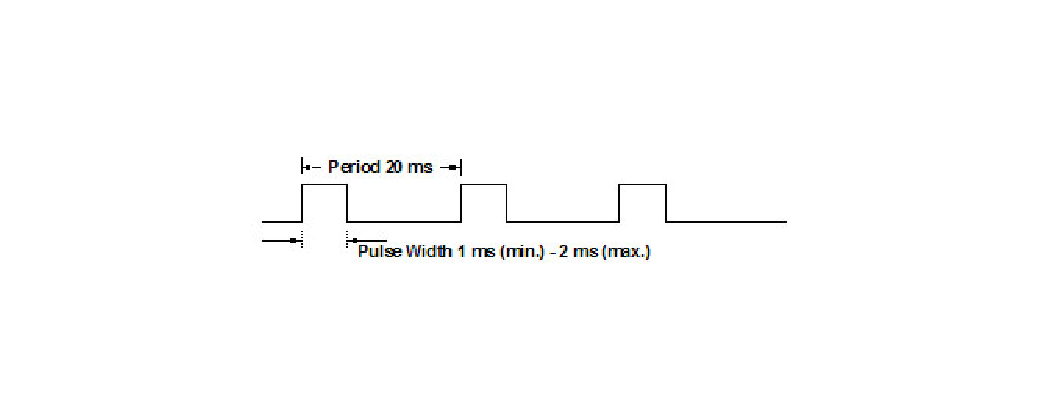
\includegraphics[width=1.0\textwidth]{figures/ServoPwm}
    \caption[Signal modulé]{\label{ServoPwm}Schéma de la modulation du signal
      \'electrique \protect
      \cite{WikiServo}
    }
\end{figure}

Comme l'on peut voir, le dit signal, est form\'e de hauts et de
bas. Lorsqu'il est ``bas'', cela veut dire que la tension est basse ou égale
à 0V. Lorsqu'il est
``haut'', cela veut dire que la tension est a une valeur définie auparavant,
standard, différente de 0V. Dans notre cas, le ``haut'' est à 5V (standard
pour le modélisme et l'électronique en général). On appelle la
période pendant laquelle le signal est ``haut'' une pulsation.

Chaque début de pulsation est séparé par un temps bien défini de
20ms. Ce qui peut varier d'une pulsation \`a l'autre, donc ce qui informe le
servo-moteur en quel angle il doit se positionner, est la longueur de la
pulsation. Comme indiqué, celle-ci peut varier de 1ms \`a 2ms.

\subsection{Programmation pour contr\^oler un servo}
Le programme se trouvant en annexe (\ref{SketchExServo}) est un exemple propos\'e dans la section
``apprentissage'' du site officiel d'Arduino \cite{ServoSweep}. Il utilise la librairie
``Servo'' installée avec l'IDE Arduino. Ce que font les méthodes de cette
classe est de produire un signal comme celui discuté à la section
précédente en l'émettant par un des pins de l'Arduino capable de cette
modulation. 

%--------------- Temporaire ---------------%
% Il ne faut pas oublier de parler de ce problème!!!!
\subsection{Etat actuel du système de guidage}
Le servo-moteur n'est pas fonctionnel sur la plaque électronique que nous avons conçu
nous-même. Selon nos diagnostiques, il s'agit d'une mauvaise soudure et donc
le servo-moteur ne peut pas être alimenté en courant. Ce problème devrait se
résoudre lorsque nous recevrons le PCB.


D'ailleurs, ce programme est tr\`es pratique pour tester le fonctionnement d'un servo-moteur. 

\section{Moteur de propulsion}

\subsection{Descriptif}

Le moteur de propulsion, au contraire du servo, n'a pas été changé.
 Ses caractéristiques électriques (données que nous avon mesuré à l'aide
d'un multimètre du gymnase) se trouvent \`a la section
(\ref{TableDesc}). Le moteur est muni d'une boite \`a vitesse ainsi qu'un
différentiel. Nous avons estimé qu'il aurait été
inutilement compliqué d'y apporter des modifications. La
configuration déjà existante, à l'exception de l'éléctronique
subvient tout à fait à nos besoins.  

\subsection{H-bridge}\label{h-bridge}
Faire tourner l'axe d'un moteur \'electrique pose peu de probl\`emes. Il
suffit de connecter l'un des p\^oles \`a la tension positive et l'autre \`a la tension
n\'egative. Ceci fera tourner l'axe du moteur dans un sens. Si vous souhaitez le
faire tourner dans le sens inverse, il vous suffira d'\'echanger les fils
\'electriques aux p\^oles du moteur.

Le probl\`eme suivant se pose alors: comment inverser le sens de marche du
moteur sans intervention manuelle?

La r\'eponse est donn\'ee par un astucieux circuit compos\'e de
transistors. Il permet, au moyen de deux signaux actionnant les transistors,
de contr\^oler le sens du courant passant dans le moteur.

Le schéma suivant pourra d'avantage \'eclairer le lecteur.

\begin{figure}[h]
\centering
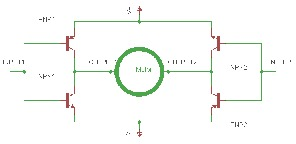
\includegraphics[width=1.0\textwidth]{figures/H-bridge}
    \caption[H-Bridge]{\label{H-bridge}Sch\'ema d'un H-bridge}
\end{figure}

\textbf{Explications}

Pour fabriquer un H-bridge, il faut utiliser entre autres des transistor NPN \footnote{Négatif-Positif-Négatif} et PNP \footnote{Positif-Négatif-Positif}.  La diff\'erence pratique
entre ces deux types de transistors est que l'un demande un signal
d\'eclencheur haut pour \^etre ouvert tandis que l'autre en demande un
bas ou la terre. Dans ce cas, on utilise deux types de transistors
diff\'erents (en grande partie pour clarifier le sch\'ema), mais l'on pourrait
tr\`es bien utiliser uniquement des transistors du m\^eme type. On obtiendrait
le m\^eme r\'esultat en connectant les \emph{INPUT} \`a des transistors
diagonalement oppos\'es\cite{RobotRoom}.

On peut voir que selon le \emph{INPUT}, on obtiendra des tensions au bornes du
moteur ou \emph{OUTPUT} variables.
\subsubsection{Table de V\'erit\'e}
R\'edigeons un tableau de v\'erit\'e pour mieux illustrer la situation, o\`u H
(\textit{high}) signifie haut et L (\textit{low}) signifie bas :


\begin{table}%[!h]
\begin{center}
  \begin{tabular}{c|c||c}  
    \emph{INPUT1} & \emph{INPUT2}
    & Tension\\
    \hline
    H & L & \emph{OUTPUT1} $=$ \emph{OUTPUT2}\\
    L & H & \emph{OUTPUT1} $=$ \emph{OUTPUT2}\\
    H & H & \emph{OUTPUT2} $>$ \emph{OUTPUT1}\\
    L & L & \emph{OUTPUT1} $>$ \emph{OUTPUT2}\\
  \end{tabular}
\end{center}

\caption[Table de v\'erit\'e, H-Bridge]{\label{tableDeVerite} Table de v\'erit\'e accompagnant le sch\'ema du
H-bridge (fig: \ref{H-bridge})}

\small Quand les signaux \emph{INPUT} sont oppos\'es, le moteur est \`a
l'arr\^et. Quand ils sont \'equivalents, le moteur est en marche, dans un sens
ou dans l'autre.\normalsize
\end{table}


\section{Coût des composants}
Le tableau \ref{TableCout} contient les éléments clefs que nous avons utilisé pour construire notre drone.

\begin{centering}
\begin{table}
\begin{tabular}{| l | c | r |}
\hline
Composant & Quantité & Prix [CHF] \\
\hline
Voiture radio-commandée & 1 & 30.00\\
\hline
Arduino Uno & 1 & 20.00 \\
\hline
Raspberry Pi& 1 & 35.00 \\
\hline
Batterie externe (7000mAh) &1 & 28.00 \\
\hline
Webcam & 1 & 35.00\\
\hline
Edimax EW7811Un (wi-fi) & 1 & 18.40\\
\hline
Hub USB & 1 & 5.60\\
\hline
Capteur de distance (HC-SR04) & 1 & 3.20\\
\hline
L293D & 1 & 3.00\\
\hline
Câble micro USB & 1 & 1.40\\
\hline


\hline
\hline
total & 10 & 179.60\\
\hline

\end{tabular}
\caption{\label{TableCout}Synthèse des composants clef, leur prix et le prix total.}
\end{table}
\end{centering}





\chapter{Software \\  Première version des systèmes embarqués}
%\addcontentsline{toc}{chapter}{\protect\numberline{}\normalsize Software Première version des systèmes embarqués}

\section{Software de l'Arduino}
\lettrine{P}{our} programmer l'Arduino, nous utilisons le logiciel dédié, \textit{Arduino IDE}\footnote{IDE signifie \textit{Integrated Development Environment}. C'est une ensemble d'outils qui sont mis à la disposition des programmeurs afin de simplifier et augmenter leur productivité.} (fig: \ref{Environnement Arduino}). C'est un environnement \textit{open source}\footnote{Terme de \textit{Open source}\cite{openSource} signifie littéralement "Libre de droits", ceci indique donc qu'un logiciel \textit{Open source} permet à n'importe qui d'avoir accès au code source dans son intégralité. "L'Open Source est un monde de partages où chacun peut apporter une pierre à l'édifice pour améliorer encore et toujours les solutions retenues"\cite{OpenSourceCit}} qui fonctionne sur Windows, Linux et Mac OS X. Il a été écrit en Java et est basé sur le logiciel Processing.
\begin{figure}[h!]
\begin{center}
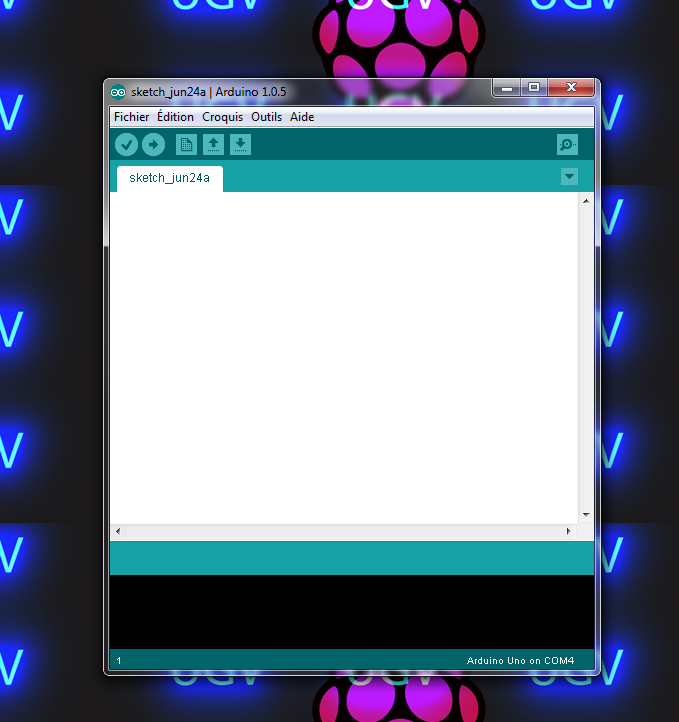
\includegraphics[scale=0.5]{arduino-environnement-1}\\
\caption[Environnement de programmation Arduino]{Environnement Arduino\label{Environnement Arduino}, C'est la fenêtre qui nous permet d'écrire un code dans un pseudo C, de le compiler et le téléverser sur l'Arduino. Ce programme a un sorte de petit déboggeur qui est très basique, mais très souvent suffisant.}
\end{center}
\end{figure}
Ce logiciel nous permet de programmer, de compiler et de téléverser un code à un Arduino. Il possède aussi des exemples de codes afin de pouvoir apprendre à utiliser un Arduino sans avoir à chercher sur le web. Il prend en compte des librairies qu'on peut rajouter simplement en mettant la librairie dans le dossier "\textit{\textbackslash arduino\textbackslash librairies}". Ce software permet aussi à l'utilisateur d'envoyer des caractères ou des chaînes de caractères à l'Arduino par le biai du port \textit{Serial}, il faut néanmoins appuyer sur entrée pour envoyer le caractère ou la chaîne de caractères.


\section{Software du Raspberry Pi}

Sans les logiciels, notre projet aurait bien du mal à se réaliser. Dans cette section, nous allons parler de tout les softwares que nous utilisons sur la Framboise pour la première version du drone. Dans un premier temps, nous allons rapidement aborder la question du sans fil et de la connexion que nous avons mise en place afin de contrôler le drone, avant de continuer sur le logiciel Guvcview, qui permet d'afficher une image. Par la suite, nous allons brièvement parler de notre programme python qui permet de contrôler le véhicule avant de finir le chapitre avec un résumé de points forts ou moins forts de cette première version.




\subsection{Sans fil}

Au niveau hardware, afin que le Raspberry Pi puisse se connecter sur le réseau sans fil, nous utilisons un \textit{dongle} (fig:\ref{Edimax}) Wi-Fi \footnote{Le modèle utilisé est le suivant: EW7811Un fabriqué par Edimax}. Cet accessoire ne nécessitant pas de \textit{driver} \footnote{Un driver est un petit logiciel permettant d'exploiter le Hardware},il est donc directement reconnu et peut rapidement être configurer par le Raspberry Pi. 
\begin{figure}[!h]
\begin{center}
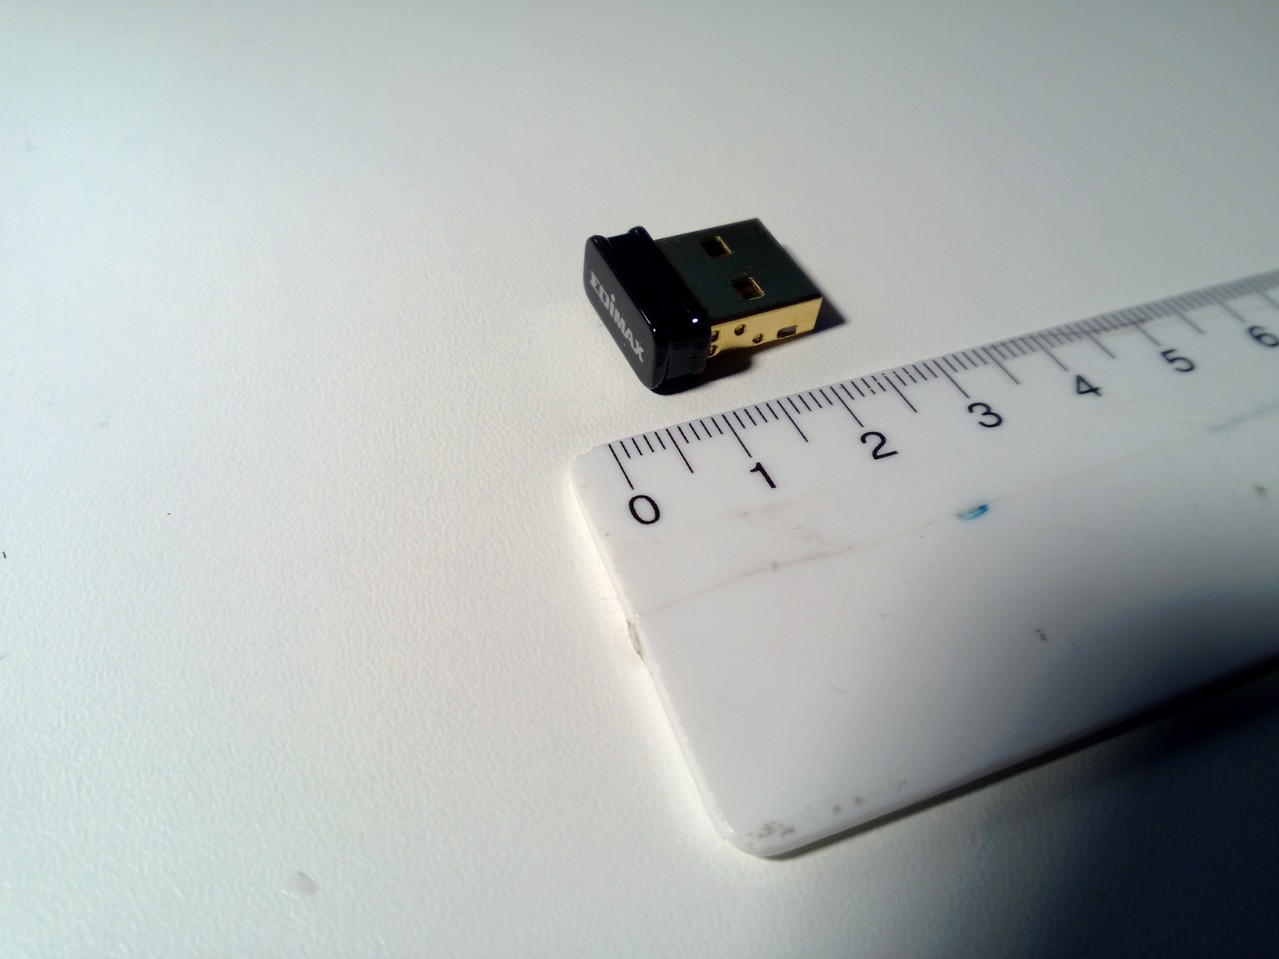
\includegraphics[scale=0.38, trim=300 300 300 0, clip=true]{Edimax}
\caption[\textit{Dongle} Edimax EW7811Un]{\textit{Dongle} Edimax EW7811Un. Connecté par USB à la Framboise, il permet au Raspberry Pi de se connecter via Wi-Fi à une borne\label{Edimax}}
\end{center}
\end{figure} 

\subsubsection{Partage sécurisé}

Au niveau software, nous utilisons un type de partage sécurisé entre deux ordinateurs, qui se nomme \textit{ssh} pour \textit{Secure Shell}. C'est un protocole permettant à un ordinateur de faire une connexion sécurisée avec un autre afin de le contrôler. Meilleur que VNC (\textit{Virtual Network Computing}) dans le sens où il ne demande pas au Raspberry Pi de dupliquer le \textit{Desktop} (bureau), ce qui nous permet d'améliorer les performances, tant du côté de la réactivité des commandes, que du nombre d'images par secondes de la caméra envoyées par le Raspberry Pi. Il y a deux inconvénients majeurs à ces solutions, la première, c'est qu'il faut établir la connexion et lancer les programmes manuellement. Le deuxième inconvénient, c'est qu'il est beaucoup plus compliqué, voire impossible à un utilisateur n'utilisant pas un système UNIX de se connecter au Raspberry Pi. Ce qui fait en sorte que notre drone ne toucherais pas un grand public.

\subsection{Guvcview}

Guvcview\label{Guvcview} est un software permettant d'enregistrer des séquences vidéos ou des images, il fournit aussi une image de contrôle, que nous utilisons dans la première version du drone. Ce logiciel très facile d'utilisation permet d'avoir près de sept images par secondes lors d'une connexion \textit{ssh} avec une résolution d'environ 240x160 pixels. L'inconvénient de ce logiciel est que l'image de contrôle ne peut pas être affichée seule, elle s'accompagne toujours du panneau de réglages. De plus, il y a un temps de latence d'environ 700ms. 

\section{Python}
Outre les programmes mentionnés ci-dessus, nous avons développé notre propre
code python (annexe: \ref{code python}) qui permet de contrôler le
véhicule. L'interface graphique est très simple
(fig: \ref{python environnement}). Il s'agit simplement d'une fenêtre qui est à
l'écoute du clavier et qui, lorsque l'utilisateur presse une touche, va
envoyer le caractère à l'Arduino via le port de communication
\textit{Serial}. L'Arduino va ensuite, grâce à son propre code définir quelle action le
véhicule doit faire. Ce programme permet non seulement de choisir la direction
à prendre, mais aussi de régler l'angle de braquage ou la vitesse maximale. Il
affiche entre autre les messages d'erreur ainsi que des informations à propos
de la vitesse maximale ou du braquage maximal. Ce programme ne prend pas en
compte l'utilisation de capteur, tel que capteur de distance. Il permet
simplement de diriger le véhicule. Une zone de texte non éditable par
l'utilisateur permet d'afficher des messages, avertissant, par exemple, que le
pilote a atteint le braquage maximal. Le programme n'est pas conscient de
l'état physique de la voiture, mais se base uniquement sur les paramètres
sélectionnés par le pilote pour imprimer de tels messages. 

\begin{center}
\begin{figure}[!h]
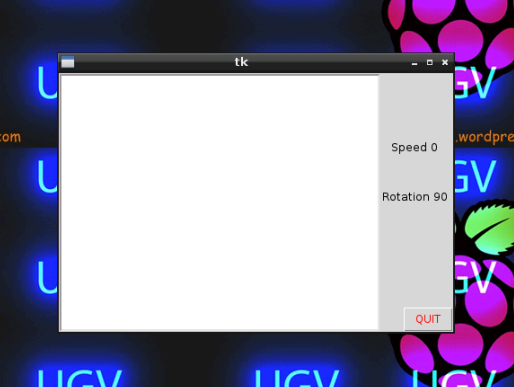
\includegraphics[scale=1]{python-environnement}\label{python environnement}
\caption[Interface graphique Python]{Fenêtre X du code python qui permet la lecture du clavier. Cette fenêtre permet de contrôler le drone. Le programme affiche sud la colonne de droite l'angle de rotation des roues ainsi que la vitesse maximale du drone.}
\end{figure}
\end{center}


\section{Évaluation de la première version}

Avant de commencer à parler de la deuxième version, nous allons analyser quels sont les points forts ou points faibles de cette première version. Les avantages de cette versions sont surtout au niveau des programmeurs. En effet, cette version est assez simple à programmer, dans le sens où nous utilisons déjà des programmes qui existent déjà et nous nous sommes surtout occupé de l'interface humain machine. Les communications (ssh ou serial) sont très simple a utiliser. Les inconvénients se placent surtout au niveau de l'utilisateur. En effet, il n'est pas très pratique de devoir ouvrir un Terminal, se connecter au drone via ssh, lancer trois programmes manuellement avant de pouvoir utiliser le drone. De plus, la connexion cryptée fait baisser la rapidité de la connexion (qui est surtout visible avec l'image de la caméra). C'est pourquoi nous nous sommes lancés dans une deuxième version du drone, qui, en plus d'avoir de nouvelles fonctions, est plus simple d'utilisation et plus fluide. 

\clearpage

\chapter{Software \\ Deuxième version des système embarqués}

\lettrine{D}{ans} notre projet, nous avons prévu une deuxième version du drone, 
dans le sens où la première version ne remplissait pas tout à fait les buts que nous 
nous étions fixés. Cette version, principalement programmée en Java et en C++, 
nous permet de faire nous même la connexion entre l'ordinateur et le Raspberry Pi. Le C++ a été utilisé dans tout ce qui touche la caméra. Il a été choisi car il est beaucoup plus rapide que le Java, et donc essentiel au niveau de l'image, où nous cherchons les meilleures performances. Le reste à été codé en Java. Nous avons choisis ce langage pour plusieurs raisons. Tout d'abord, nous avions des notions en Java, 
ce qui n'est pas négligeable quand on doit choisir un programme, c'est aussi un langage constamment mis à jour et il possède une large communauté, ce qui fait que de nombreuses classes existent, notamment du côté des interfaces graphiques,
sans lesquelles nous aurions de la peine à rendre le programme agréable à utiliser. Dans ce chapitre, nous allons tout d'abord aborder le type de structure employée et le choix de protocole
que nous avons adopté, nous allons ensuite voir à quoi ressemble notre programme Java et ce qu'il fait. Avant de parler
de la vidéo avec le programme en C++ ainsi que OpenCV.
langage constamment mis à jour et il possède une large communauté, ce qui fait
que de nombreuses classes existent, notamment du côté des interfaces graphiques,
sans lesquelles nous aurions de la peine à rendre le programme agréable à 
utiliser. Dans ce chapitre, nous allons tout d'abord aborder le type de structure employée et le choix de protocole
que nous avons adopté, nous allons ensuite voir à 
quoi ressemble notre programme Java et ce qu'il fait. Avant de parler
de la vidéo avec OpenCV. 


\section{Client/Serveur\label{ClientServeur}}
Le model client-serveur est composé de deux partis: les serveurs qui fournissent un service et les clients qui bénéficient de celui-ci. Un client ne partage pas ses ressources avec les autres, mais profite de celles du serveur. Le Serveur attend qu'un client vienne se connecter et faire des requêtes auxquels il répond. Il doit généralement être capable de gérer plusieurs clients à la fois.

\begin{figure}[h]
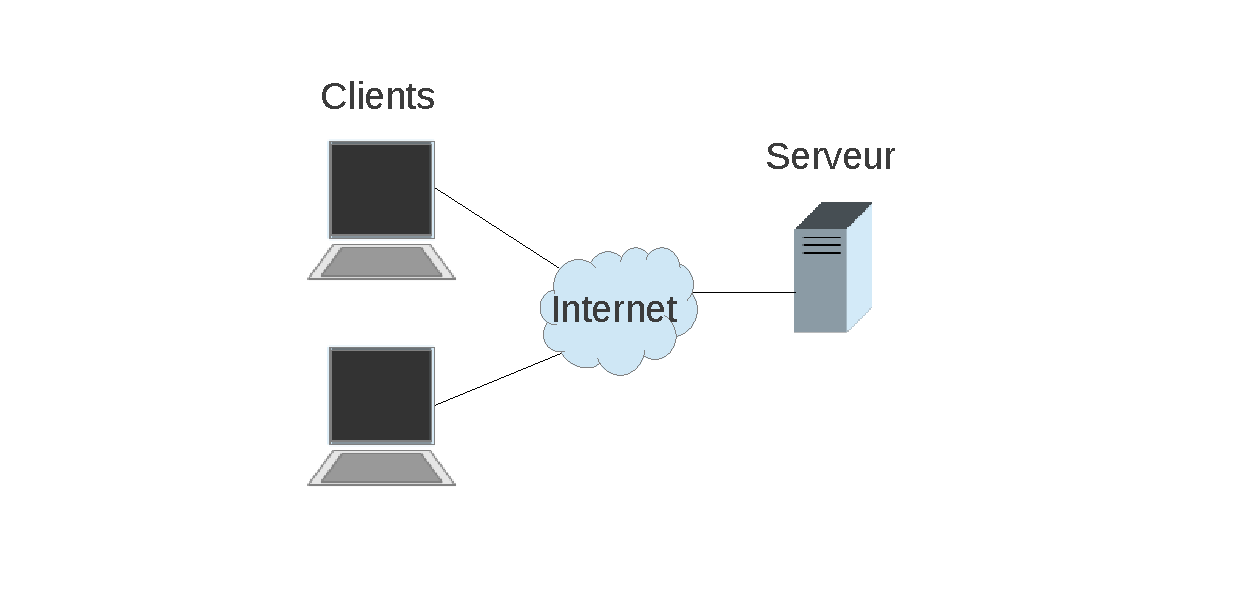
\includegraphics[width=1.0\textwidth]{figures/Client_Server1.pdf}
\caption[Structure client-serveur]{\label{ClientServer1}Structure client-serveur.}
\end{figure}

Nous avons établi que la voiture occupe le rôle de serveur qui est exécuté sur le RaspberryPi. Il contrôle les mouvements de la voiture par l'intermède de l'Arduino. Le client peut être n'importe quelle machine sur le réseau local utilisant le côté client du code. Le code est effectivement constitué de deux "main class", c'est à dire des applets, "Server" et "Client". 

Un Thread est initié pour chaque nouvelle demande de connexion. C'est à dire que le serveur peut s'occuper en parallèle des requêtes de différents clients (voir fig. \ref{ClientServer2}). 

\begin{figure}[h]
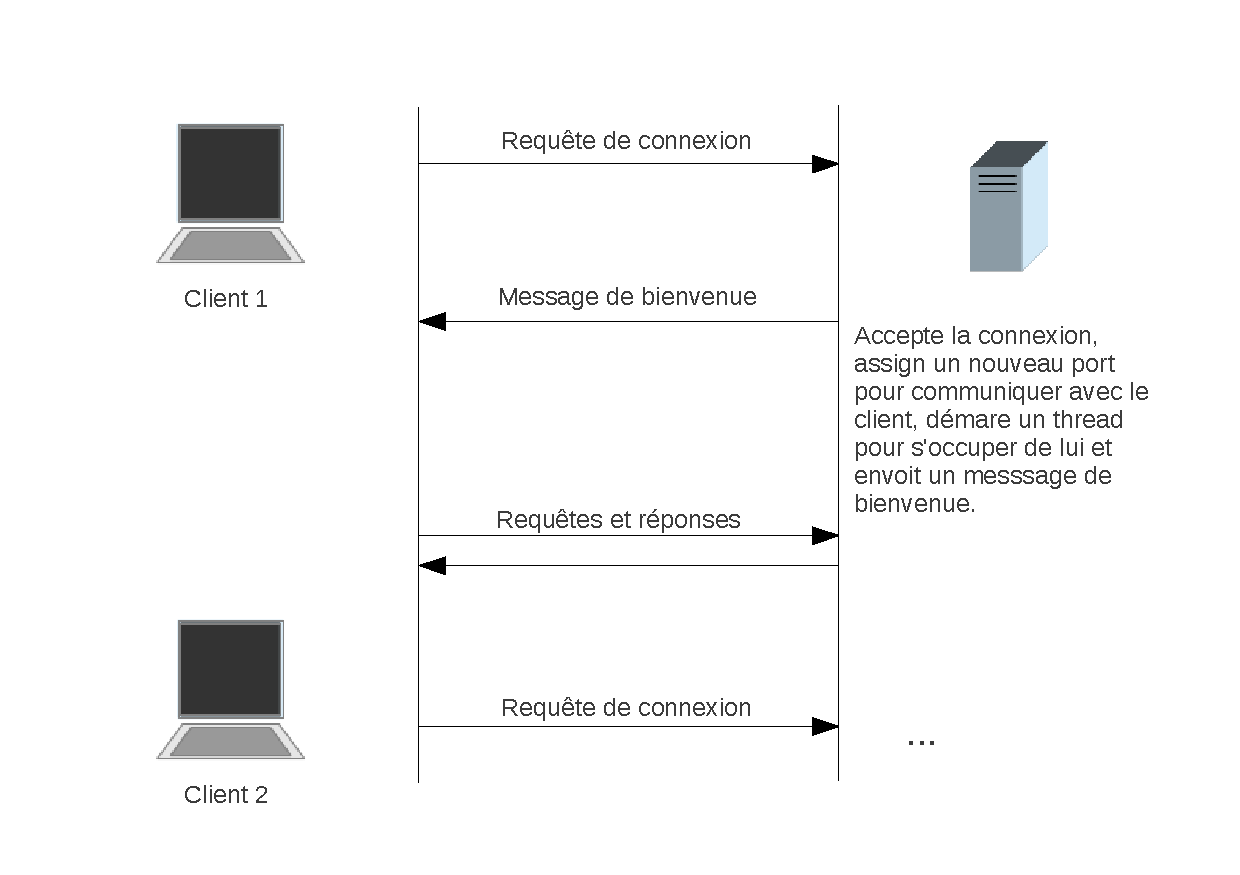
\includegraphics[width=1.0\textwidth]{figures/Client_Server2.pdf}
\caption[Connexion d'un nouveau client]{\label{ClientServer2}Schéma de la procédure suivie à chaque nouvelle connexion.}
\end{figure}


\section{UDP ou TCP\label{UDPTCP}}
Avant de parler de notre choix, nous allons un peu expliquer ce que sont les protocoles UDP et TCP et leurs différences. UDP et TCP sont deux protocoles de connexion réseau qui permettent d'envoyer des données, (\textit{Packets}), d'un ordinateur à un autre.

e protocole UDP\footnote{\textit{User Datagram Protocol}, soit protocole des datagrammes d'utilisateurs} est un protocole qui n'est pas orienté connexion. Les paquets qui transitent via un protocole UDP ont l'adresse IP du récepteur, comme la poste, mais il n'y a aucune garantie que les paquets soient bien arrivés sans parler de leur ordre. Par contre, il n'y a pas le souci de perte de connexion puisque il n'y en a pas. Ce protocol est particulièrement adapté pour la transmission de vidéo. Pour contrôler les mouvements du véhicule il est impératif qu'il sache à tous moment si il y a au moins un client qui est au contrôle, au risque que le véhicule soit livré à lui même. Ici rentre en jeu le protocole TCP. 

Le protocole TCP\footnote{\textit{Transmission Control Protocol}, soit protocole de contrôle des transmissions} est l'opposé de l'UDP, il est orienté connexion. Lorsque le client envoie des données au serveur, ce premier est informé de l'arrivée des dites données. Il y a donc un système de reçu qui confirme la réception des packets. S'il y a des fichiers corrompus, l'expéditeur va renvoyer les fichiers manquants. On peut, par analogie, comparer ce protocole à la communication téléphonique. On remarque assez rapidement quand il y a une coupure dans la ligne.\\

\section{Java}
Le code complet Java est très long et est composé de beaucoup de classes. Plutôt que de tout détailler ou pire, juste mettre le code cru, nous avons sélectionné les thèmes les plus intéressants que nous avons rencontré pendant l'écriture du programme. Nous allons expliquer comment nous avons structuré le système, selon l'architecture et le protocole discutés en section \ref{ClientServeur} et \ref{UDPTCP}.

\subsection{Gestion des Requêtes de connexion}
Pour établir une connexion avec le serveur, un client va ouvrir un port de communication avec les serveur, appelé "Socket". Une fois cette opération complétée avec succès, il sera possible d'obtenir les "Streams"\footnote{Tuyau pour transmettre des bytes} entrant et sortant pour effectivement envoyer des données.

\lstinputlisting[language=Java]{code/JavaExConnection.txt}

De l'autre côté, le serveur attend les demandes de connexion, ceci grâce à la classe welcomeSocket qui s'occupe de ce genre de requêtes. Une fois la requête de connexion acceptée le socket de communication est récupéré et un thread est lancé avec en argument le socket de communication pour pouvoir poursuivre l'échange de données. Finalement, le thread est stocké dans une liste, ainsi quand le serveur doit envoyer un message aux clients il itère simplement à travers la liste de thread.

 \lstinputlisting[language=Java]{code/JavaExConnectionServer.txt}
 
 Puisque il est dans une boucle while, il se remet en attente de la prochaine requête.
 
 \subsection{gestion des Requêtes suivantes}
 Le Client dispose d'une variété de requêtes prédifinies. A titre d'exemple on va définir des pseudos requêtes avancer, reculer et s'arrêter. De plus, lié à la requête vient s'ajouter une option pour donner plus de précision sur, dans ce cas, la vitesse. Une pseudo requête se présenterait alors sous cette forme:
 
 \indent{Avancer(20)}
 
 Ce qui voudrait dire: "Rouler vers l'avant à 20cm/s".  Pour bien comprendre la demande d'un client le serveur a également cette même liste de requêtes prédéfinies dont il sait s'occuper. Une fois que le serveur a trouvé la requête dans sa liste, il exécute l'opération prévue pour cette situation. Le schéma \ref{RequestHandler} illustre cette procédure.
  Le tableau de requêtes est enfait un HashMap, les identifiants des requêtes se trouvent à gauche en majuscule et les références aux fonctions à exécuter se trouvent à droite.
 
 \lstinputlisting[language=Java]{code/JavaExRequestList.txt}
 
 \begin{figure}[!h]
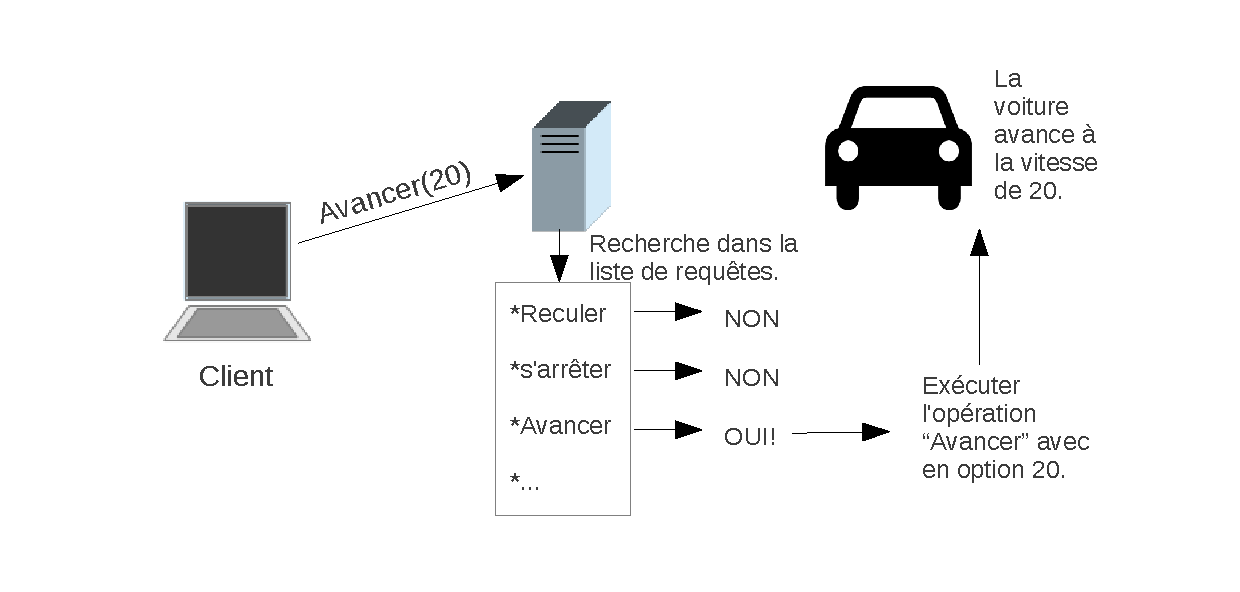
\includegraphics[width=1.0\textwidth]{figures/RequestHandler.pdf}
\caption[Gestion de requête au serveur]{\label{RequestHandler}Schéma de la procédure suivie pour une requête au serveur.}
\end{figure}
 
\subsection{librxtx}

Afin de pouvoir communiquer entre l'Arduino et le RaspberryPi via USB, nous avons fait appel à une librairie java supplémentaire qu'il a fallu installer. librxtx s'occupe de gérer les ports de communication usb et d'effectivement établir une communication avec un appareil connecté par ce moyen.

Grâce à cette librairie nous avons pu écrire notre propre classe qui permet de facilement sonder le système pour un appareil tel que l'arduino, établir une connection à cette appareil et lui envoyer des données. Le système de réception de messages usb est basé sur un model évènementiel, expliqué dans la section \ref{Event}.

\subsection{Evènements usb et écoute d'un Stream\label{Event}}

La programmation événementielle permet dans certains cas d'améliorer l'efficacité d'une application. Elle est basée sur des évènements ou changements d'états qui déclenchent des autres morceaux de code. Ce type de programmation s'oppose à la programmation dite séquentielle.

Pour illustrer cette architecture, imaginons deux téléphones, l'un est dépourvu de haut-parleurs (voir fig.\ref{ChatExample}). Pour chatter, l'utilisateur du téléphone déféctueux devra régulièrment contrôler si il a reçu un nouveau message et souvent il contrôlera pour rien, tandis que l'autre sera averti d'un nouveau message (changement d'état, événement!) et contrôlera uniquement à ce moment là.  

\begin{figure}[h]
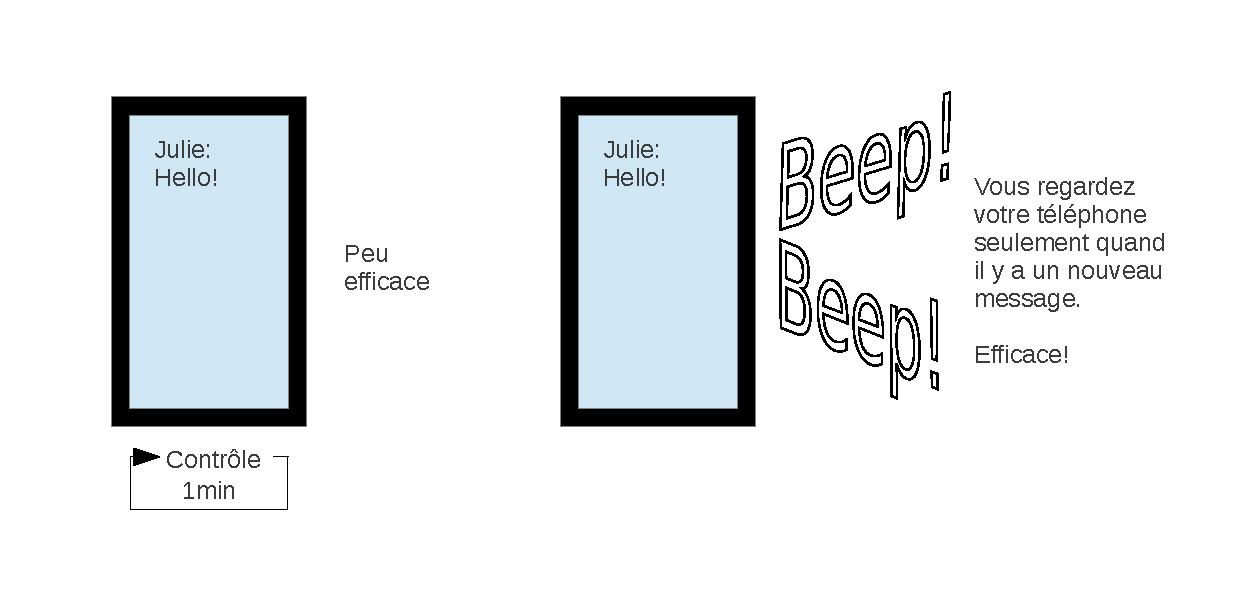
\includegraphics[width=1.0\textwidth]{figures/EventProgramming1.pdf}
\caption[Analogie à la programmation événementielle]{\label{ChatExample}L'utilisateur du téléphone sans haut-parleur contrôlera régulièrement son téléphone et souvent pour rien.}
\end{figure}

Notre code java utilise ce système pour tout ce qui concerne la réception de message, donc l'écoute de Stream, c'est à dire que dès qu'un message est reçu, aussi bien par le client que par le serveur, le code pour gérer ce message est exécuté. L'interface graphique (GUI) est basée par principe sur des événements, par exemple: "boutton pressé", "champ de text modifié", "touche enfoncée".

\begin{figure}[h]
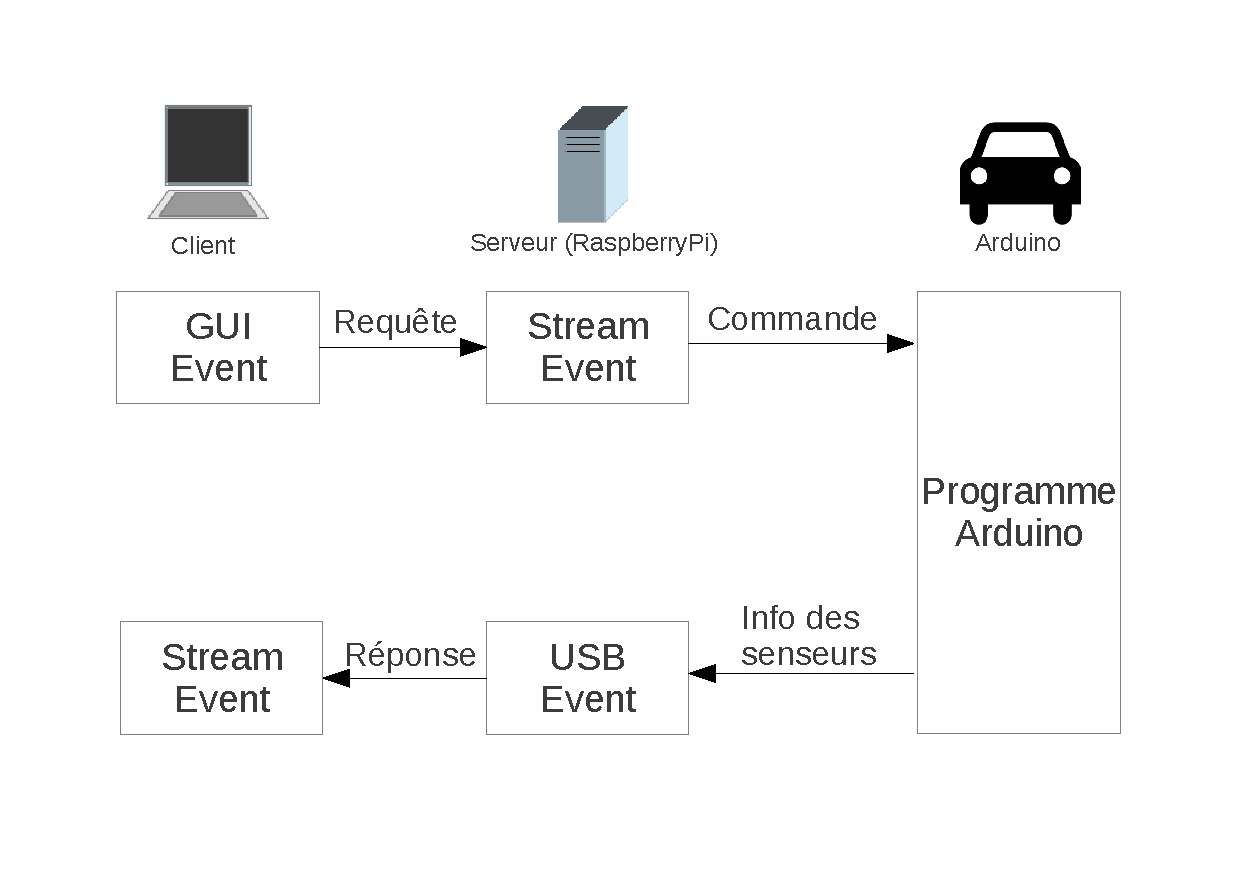
\includegraphics[width=1.0\textwidth]{figures/EventProgramming2.pdf}
\caption[Evénements dans notr architecture]{\label{SuiteEvent}Cette figure illustre la suite d'événements possible dans l'architecture de notre projet}
\end{figure}
\section{C++ et vidéo}

Après avoir parlé de ce que faisait notre code Java, nous allons ici aborder la partie touchant à la vidéo, et par conséquent, au code C++.  Comme dit précédemment, nous utilisons le protocole de réseau UDP  pour transmettre la vidéo. La raison du choix de ce langage réside dans le fait que c'est un langage qui est exécuté beaucoup plus rapidement que un langage de haut niveau tel que Java (la communauté considère que cette différence de rapidité équivaut à un facteur trois). Le programme en C++ est un programme invisible par l'utilisateur. En effet, il fonctionne en arrière plan. Voici le plan du programme:
\begin{enumerate}
\item Ouverture d'une socket du côté du Raspberry Pi et de l'ordinateur distant
\item Capture du flux vidéo de la caméra connectée à la Framboise
\item Compression du flux video
\item Envoi du flux vers l'ordinateur distant
\item Réception et décompression des packets reçus
\item Affichage de l'image dans le programme Java
\end{enumerate}



\subsection{Client serveur}

Nous allons maintenant aborder une petite présentation du code pour comprendre comment fonctionne notre client serveur. Par soucis de simplicité, nous n'allons que parler du code écrit pour Windows. Mais nous avons annexé le code fonctionnant avec les système UNIX en annexe [annexe à venir].
%TODO Rajouter l'annexe du code client serveur en c++ pour UNIX

Tout d'abord, il faut indiquer quelles librairies nous utilisons, c'est les lignes suivantes. La première ligne permet d'utiliser les socket Windows. Les autres lignes sont des librairies standards en C++.
\lstinputlisting[language=C++, firstline=3, lastline=6]{code/client-exemple.cpp}

Une fois que ceci est fait, nous initialisions quelques variables dont il n'est pas utile de préciser à quoi elle vont servir. Ensuite, nous initialisons deux objets aux deux lignes ci-dessous. Nous verrons un peu plus tard à quoi elle servent. 
\lstinputlisting[language=C++, firstline=16, lastline=17]{code/client-exemple.cpp}
Le premier objet va se voir attribuer les données contenues dans la fonction \textbf{socket()}
\lstinputlisting[language=C++, firstline=34, lastline=35]{code/client-exemple.cpp}
La fonction \textbf{socket(famille, type, protocole)} possède 3 arguments. Le premier, \textbf{AF\_INET} est la famille de protocole utilisée, elle utilise une adresse internet IPV4, c'est a dire qui est encapsulée sur 4 octets. Le deuxième argument détermine le type de communication à faire, dans notre cas, \textbf{SOCK\_DGRAM} signifie que nous sommes en UDP. Le troisième argument permet de spécifier un protocole qui permet de fournir un service désiré, dans notre cas, nous n'avons besoin de rien, il est donc à $0$. \textbf{socketId} va donc recevoir les argument de la fonction \textbf{socket()}. Ils seront utilisés un peu plus tard.\\

\lstinputlisting[language=C++, firstline=43, lastline=45]{code/client-exemple.cpp}



\subsection{OpenCV}




\clearpage

\appendix

\section{Sketchbook}

%\subsection{Sketch exemple pour le moteur}
%\lstinputlisting[language=Java]{code/motor.java}
%
%\subsection{Sketch exemple pour le servo \label{SketchExServo}}\cite{ServoSweep}
%\lstinputlisting[language=Java]{code/ServoExample.java}
%
%\textbf{Commentaires}
%
%On commence par inclure la classe Servo, puis on crée un objet
%\emph{Servo}. Dans la fonction \emph{setup} du programme, on lie l'objet
%\emph{myservo} au pin neuf de l'arduino. Ensuite, dans la fonction \emph{loop}, on
%fait varier la position du servo grâce \`a la méthode \emph{write}. Un
%d\'elai (le programme s'arrête en ce point) de 15ms pour permettre au servo-moteur
%d'atteindre la position demandée. Etant donnée que cette opération est
%ittérée plusieurs fois au moyen d'une boucle \emph{for}, on pourra voir le
%servo décrire un mouvement de balayage.
%
%\subsection{Code python sur le Raspberry Pi \label{code python}}
%\lstinputlisting[language=python]{code/gui_1.1.py}




\bibliographystyle{plain}
\bibliography{references}


%}

\end{document}

\end{document}
